\documentclass[10pt,aps,pra,reprint,amsmath,amsfonts,amssymb,showpacs]{revtex4-1}
\usepackage{epsfig,psfrag,graphicx,bm,color}

\def\del#1{{}}
%\def\del#1{{\bf (DELETED TEXT)}}
\def\C#1{#1}
%\def\C#1{{\bf #1}}


% --- journals --- %
\newcommand{\aap}{A{\&}A}
\newcommand{\aaps}{A{\&}AS}
\newcommand{\aj}{AJ}
%\newcommand{\apj}{ApJ}
\newcommand{\apjl}{ApJL}
\newcommand{\apjs}{ApJS}
\newcommand{\apss}{Ap{\&}SS}
\newcommand{\araa}{ARA{\&}A}
%\newcommand{\prd}{Phys. Rev. D}
%\newcommand{\pre}{PRE}
\newcommand{\mnras}{MNRAS}
\newcommand{\ssr}{SSRv}
%\newcommand{\nat}{Nature}
\newcommand{\physrep}{Phys.~Rep.}
\newcommand{\jcomp}{J.~Comput.~Phys.}
\newcommand{\jcap}{JCAP}

%NEW
\newcommand{\rmn}{\mathrm}
\newcommand{\bx}{{\bf x}}
\newcommand{\fg}{{F_\gamma}}
\newcommand{\sg}{{S_\gamma}}
\newcommand{\psf}{\theta_\rmn{res}}
\newcommand{\ph}{\rmn{ph}}
\newcommand{\eph}{E_\ph}
\newcommand{\nph}{N_\ph}
\newcommand{\vir}{\rmn{vir}}
\newcommand{\gal}{\rmn{gal}}
\newcommand{\sd}{\rmn{SD}}
\newcommand{\clu}{\rmn{cl}}
\newcommand{\sfe}{\rmn{sfe}}
\newcommand{\sub}{\rmn{sub}}
\newcommand{\msun}{M_\odot}
\newcommand{\ee}{E_\rmn{e}}
\newcommand{\stars}{\rmn{stars}}
\newcommand{\dust}{\rmn{dust}}
\newcommand{\lx}{L_\rmn{X}}
\newcommand{\s}{\rmn{s}}
\newcommand{\Kp}{\rmn{K}^\prime}
\newcommand{\Ip}{\rmn{I}^\prime}
\newcommand{\Js}{\rmn{J}^*}
\newcommand{\Jp}{\rmn{J}^\prime}
\newcommand{\B}{\rmn{B}}
\newcommand{\bsub}{\B_\rmn{sub}}
\newcommand{\qCR}{q_{\rmn{CR}-\ensuremath{\pi^0}}}
\newcommand{\ds}{{\sc DarkSUSY}}

%OLD
\newcommand{\beq}{\begin{equation}}
\newcommand{\eeq}{\end{equation}}
\newcommand{\gev}{\rmn{GeV}}
\newcommand{\tev}{\rmn{TeV}}
\newcommand{\ev}{\rmn{eV}}
\newcommand{\dd}{\rmn{d}}
\newcommand{\mx}{\ensuremath{m_{\chi}}}
\newcommand{\ga}{\gamma}
\newcommand{\ngamma}{\ensuremath{N_{\gamma}}}
\newcommand{\ngammaj}{\ensuremath{N_{\gamma,j}}}
\newcommand{\sigmaannv}{\ensuremath{\langle\sigma v\rangle}}
\newcommand{\sigv}{\ensuremath{\sigma_v}}
\newcommand{\ic}{\rmn{IC}}
\newcommand{\egamma}{\ensuremath{E_{\gamma}}}
\newcommand{\dic}{\rmn{dIC}}
\newcommand{\fsr}{\rmn{FSR}}
\newcommand{\CR}{\rmn{CR}}
\newcommand{\rhos}{\ensuremath{\rho_s}}
\newcommand{\rs}{\ensuremath{r_s}}
\newcommand{\rvir}{r_{200}}
\newcommand{\mvir}{M_{200}}
\newcommand{\rhoc}{\ensuremath{\rho_c}}
\newcommand{\e}{\rmn{e}}
\newcommand{\eg}{E_\gamma}
\newcommand{\ir}{\rmn{ir}}

\begin{document}

\title{Prospects of detecting gamma-ray emission from galaxy clusters:
  cosmic rays and dark matter annihilations}

\author{Anders Pinzke$^{1}$} \email{apinzke@physics.ucsb.edu} 
\author{Christoph Pfrommer$^{2}$}\email{pfrommer@cita.utoronto.ca}
\author{Lars Bergstr\"om$^{3}$}\email{lbe@fysik.su.se}


\affiliation{$^{1}$University of California - Santa Barbara,
  Department of Physics, CA 93106-9530, USA}

\affiliation{$^{2}$Heidelberg Institute for Theoretical Studies (HITS), Schloss-Wolfsbrunnenweg 33, DE - 69118 Heidelberg, Germany}

\affiliation{$^{3}$The Oskar Klein Centre for Cosmoparticle Physics, Department
  of Physics, Stockholm University, AlbaNova University Center, SE - 106 91
  Stockholm, Sweden}

\date{\today}

\pacs{95.35.+d, 95.85.Pw, 98.62.Gq, 98.65.-r, 98.70.Sa}


\begin{abstract}
... to be written...
\end{abstract}

\maketitle
\section{Introduction}

Dark matter has been searched for in direct detection experiments
\cite{Pato:2010zk}, at accelerators
\cite{Ellis:2001hv,Baer:2006ff,Khachatryan:2011tk} and also in
indirect detection experiments looking for signals in the cosmic-ray
spectra of antiprotons, positrons, neutrinos and all of the
electromagnetic spectrum from radio waves to gamma rays
\cite{Bergstrom:2009ib}. So far, the improvements in direct detection
sensitivity have put this method into focus, but the situation may
change considerably the coming few years as the CERN LHC experiments
collect data, and new gamma-ray detectors are being planned, such as
the CTA \cite{Consortium:2010bc}. In fact, it has recently been
pointed out \cite{Bergstrom:2010gh} that a dedicated ground-based
gamma-ray detector would have potential that goes far beyond that of
the other methods, depending on presently unknown parameters in the
particle physics models for dark matter.


Among the astrophysical systems which will be very interesting to
detect, and study, with coming gamma-ray detectors (Fermi, HESS,
MAGIC, VERITAS, and eventually large detectors like CTA) belong galaxy
clusters. The most promising directions in which to search for a
gamma-ray annihilation signal (from the annihilation process itself,
and also the accompanying bremsstrahlung and inverse Compton
components coming from charged particles produced in the annihilations)
are basically three:

1. The galactic centre (g.c.). This is where all numerical simulations
of cold dark matter predict the highest density. However, the detailed
dark matter density in the very central part is difficult to predict,
due a to a possibly very complicated interplay between baryons, dark
matter, and the central galactic black hole. Also, it is a very
crowded region with many gamma-ray sources like pulsars and other
supernova recants, which have to be subtracted from the data to
extract the dark matter induced signal. In fact, there is a recent
claim of an indication of a relatively light dark matter particle
contribution to the gamma-ray flux from the
g.c. \cite{2010arXiv1010.2752H}, but other hypotheses seem to work at
least as well \cite{2010arXiv1012.5839B}.

2. The dwarf spheroidal galaxies orbiting the Milky Way, like Segue-1,
Ursa Minor, Draco, Sagittarius, Sculptor, Carina or Willman-1
\cite{2009JCAP...01..016B,2010ApJ...720.1174A,2010JCAP...01..031S,2010JCAP...01..031S}. The
problem here is that the nature of many of these small, dark
matter-dominated galaxies is not entirely clear, and the velocity
dispersion estimates are based on rather small numbers of stars. Tidal
disruption and confusion with star clusters are other
complications. Thus the dark matter density profile is very uncertain
for most of them. Nonetheless, by stacking the data together from many
dwarf spheroidals these uncertainties can be made less severe, and
preliminary results from Fermi-LAT shows this method to give quite
promising results \cite{garde}.

3. Galaxy clusters. This possibility has been less studied, however we
noted in a previous Letter \cite{2009PhRvL.103r1302P} that the are
certain advantages that work in favour of this possible target for
gamma-ray detection of dark matter annihilation.  Galaxy clusters
constitute the most massive objects in our Universe that are forming
today. This causes their DM subhalo mass function to be less affected
by tidal stripping compared to galaxy sized halos that formed long
ago.  The annihilation luminosities of the DM halo component for
e.g. the Virgo cluster and the Draco dwarf scales in a way (see
\cite{2009PhRvL.103r1302P}) that the ratio of gamma-ray luminosities
from the smooth components is around 4, in favour of Virgo. In
addition, there may be a further enhancement due to substructure,
which to a large extent should be unaffected by tidal disruption, at
least in the outer regions.  According to a recent estimate
\cite{2011MNRAS.410.2309G}, more massive haloes tend to have a larger
mass fraction in subhalos.  For example, cluster size haloes typically
have 7.5 per cent of the mass within $r_{200}$ in substructures of
fractional mass larger than $10^{-5}$, which is 25 per cent higher
than galactic haloes \footnote{All halo masses and length scales in
  this paper are scaled to the currently favored value of Hubble's
  constant, $H_0 = 70\, \rmn{km~s}^{-1}\,\rmn{Mpc}^{-1}$. We define the
  virial mass $\mvir$ and virial radius $\rvir$ as the mass and radius
  of a sphere enclosing a mean density that is 200 times the critical
  density of the Universe $\rho_{\rmn{cr}}$.}.

For a satellite dwarf galaxy, however, once it is accreted by the
Milky Way, the outer regions are severely affected by tidal
stripping. The longer a satellite has been part of our Galaxy, and the
closer it comes to the center during its pericentral passage, the more
material is removed \cite{2004MNRAS.355..819G}.

In this paper, we will investigate in some more detail the potential
of several of the most promising galaxy clusters to yield an
annihilation gamma-ray yield which could be observable with present
and planned gamma-ray detectors.

For previous work related to dark matter in clusters, see, e.g.,
\cite{2006A&A...455...21C,2009PhRvD..80b3005J}. 


%***********************************************
{\bf Anders, insert your flux table for various clusters, and discuss it}

This yields Fornax ($\mvir=10^{14}\,\msun$) and Virgo
($\mvir=2.1\times10^{14}\,\msun$) \del{\cite{}} as the prime targets for DM
observations, Perseus ($\mvir=7.7\times10^{14}\,\msun$) for CR induced
emission and we additionally decide in favor of the well studied
cluster Coma ($\mvir=1.4\times10^{15}\,\msun$) for comparison.

\del{In this work we define the virial radius $\rvir$ of a halo to be
  the radius at which the mean density within is a factor $\Delta=200$
  times the critical density $\rhoc$ of the universe.}

% --- section:  --- %
\section{Theory}
\label{sect:theory}

\subsection{Astrophysics}
\label{sect:AP}

The differential photon flux within a given solid angle $\Delta
\Omega$ along a line-of-sight (los) is given by
\begin{equation}
\label{eq:dflux}
\frac{\dd \fg}{\dd \eg} \equiv \frac{\dd^3 \ngamma}{\dd A \,\dd t\, \dd
  \egamma} = \frac{1}{2}\int_{\Delta\Omega} \dd\psi \sin\psi \frac{\dd \sg}{\dd \eg}(\psi,\eg)\,,
\end{equation}
where
\begin{equation}
\label{eq:dtildeflux}
\frac{\dd \sg}{\dd \eg}(\psi,\eg) = \int_{\Delta\Omega} \dd\Omega \int_{\rm los}
\dd l\, q_{\rm sum}\left(\eg,r\right)\Lambda(\theta)\,,
\end{equation}
and $\sg(\psi, >\eg)$ denotes the surface brightness above the photon
energy $\eg$.  The integration along the line-of-sight $l$, in the
direction $\psi$ that the detector is pointing, is parameterized such
that the radius of the source $r=\sqrt{l^2+D^2-2 D l\cos\Psi}$, where
$D$ is the distance to the source from the galactic center and
$\cos\Psi\equiv\cos\theta\cos\psi-\cos\varphi\sin\theta\sin\psi$. The
angular integration $\dd \Omega= \sin\theta\dd \theta \,\dd \varphi$
is performed over a cone centered around $\psi$ and the opening angle
$\Delta \Omega$ is typically taken to be a few times the point spread
function (PSF) $\psf$. The limited angular resolution results in a
probability that a photon coming from a direction $\psi$' is instead
reconstructed to a direction $\psi$, where the underlying probability
distribution follow a Gaussian:
\begin{equation}
\Lambda(\theta)=\frac{1}{2\pi\psf^2}
\,\rmn{exp}\left[-\frac{\theta^2}{2\psf^2}\right]\,,
\quad \rmn{where}\quad \theta=\psi'-\psi \,.
\end{equation}
We denote the total differential source function by $q_{\rm
  sum}(\eg,r)$, where we include contributions from five main
processes; leptophilic DM annihilating either indirectly through
$\mu^+/\mu^-$ to $\rmn{e}^+/\rmn{e}^-$ or directly to
$\rmn{e}^+/\rmn{e}^-$ pairs that inverse Compton upscatter background
photons (LP-IC), leptophilic DM emitting final state radiation
(LP-FSR), supersymmetric DM benchmark models where annihilating
neutralinos generate $\rmn{e}^+/\rmn{e}^-$ pairs that upscatter
background photons (BM-IC) and emit a continuum as well as final state
radiation (BM-Cont), and CR proton induced $\pi^0$:s decaying into
gamma-rays (CR-$\pi^0$). The source function is given by
\begin{equation}
q_\rmn{sum} (\eg,r) = \qCR(\eg,r)+
\sum_i \,q_{\rmn{sm},i}(\eg,r)\,\B_{\rmn{tot},i}(\sigv,r)
\end{equation}
the differential CR to gamma-ray source function is denoted by
$\qCR(\eg,r)$ (see Sect.~\ref{sect:CRs} and \cite{2010MNRAS.409..449P}
for further details). The subscript $i$ runs over the gamma-ray
producing DM channels and the total differential boost factor for DM
is given by $\B_{\rmn{tot},i}(r,\sigv) =
\B_\sfe(\sigv)\,\B_{\sub,i}(r)$. It is the product of enhancement factors
from SFE $\B_\sfe(\sigv)$ (see Sect.~\ref{sect:LP}) and from
substructure enhancement over the smooth halo contribution
$\B_{\sub,i}(r) = 1+q_\sub(r)/q_{\rmn{sm},i}(r)$ (see
Sect.~\ref{sect:subst}). The DM source function from the smooth halo
for each process is written on the form:
\begin{equation}
\label{eq:q_sm}
q_{\rmn{sm},i} (\egamma,r) = \sum_j
\frac{\dd \ngammaj}{\dd E_\gamma} \Gamma_j(r)\,,
\end{equation}
where the annihilation rate density is given by 
\begin{equation}
\label{eq:ann_rate}
\Gamma_j(r) = \frac{1}{2} \left[\frac{\rho(r)}{\mx}\right]^2 
\, \sigmaannv_j\,.
\end{equation}
Here the subscript $j$ runs over all kinematically allowed gamma-ray
producing channels each with the spectrum $\frac{\dd
  \ngammaj}{\dd\eg}$ and annihilation cross-section $\sigmaannv_j$. We
denote the DM mass with $\mx$ and the DM density profile with
$\rho(r)$. Typically the universal Navarro-Frenk-White (NFW) density
profile provide a good fit to both the observed and simulated
clusters. It can be considered as a special case of the more general
5-parameter profile:
\begin{equation}
\rho(r) = \frac{\rhos}{\left(r/r_\s+\right)^\gamma
  \left[1+\left(r/r_\s\right)^\alpha\right]^\delta}\,,\quad
\delta=\frac{\beta-\gamma}{\alpha}\,,
\label{eq:rho_nfw}
\end{equation}
where a cuspy NFW profile is given by
$(\alpha,\beta,\gamma)=(1,3,1)$. The scaling radius is given by $r_\s$
and the characteristic overdensity by 
\begin{equation}
\rhos(c)=\frac{\Delta\,\rhoc}{3}\,\frac{c^3}
{\log\left(1+c\right)-c/(1+c)}\,,
\label{eq:rho_s}
\end{equation}
 where the halo mass dependent concentration parameter $c$ is derived
 from a power-law fit to cosmological simulations with $\mvir \gtrsim
 10^{10} \msun$ \cite{2008MNRAS.391.1940M},
\begin{equation}
\label{eq:cfit}
  c=3.56 \times \left(\frac{\mvir}{10^{15}\,\msun}\right)^{-0.098}\,.
\end{equation}
This mass scaling agrees well with \cite{2009ApJ...707..354Z} for
cluster-mass halos after converting the concentration definitions
according to \cite{2003ApJ...584..702H}. In this work we choose to
model the DM density by an Einasto density profile
\begin{equation}
\label{eq:dens_ein}
\rho_{\rm ein}(r) = \rho_{-2}\,\exp\left\{-\frac{2}{\alpha}
  \left[\left(\frac{r}{r_{-2}}\right)^\alpha -1 \right] \right\},\,
\alpha=0.17 \,,
\end{equation}
that is slightly shallower in the center than the conventional
Navarro-Frenk-White (NFW) profile, but provide a better fit to recent
simulated high resolution DM halos \cite{2010MNRAS.402...21N}. It
should also be noted that recent detailed galaxy cluster observations
find a core like density profile with an inner slope of $\beta=0.6$,
where $\beta\gtrsim 1$ can be ruled out to a $>95$\% confidence
\cite{2011ApJ...728L..39N}. In Eq.~(\ref{eq:dens_ein}) we denote the
density where the profile has a slope of $-2$ by $\rho_{-2}$, and the
radius by $r_{-2}$. Assuming that all the flux from an NFW profile
originate from within the scale radius $\rs=\rvir/c$, and all the flux
from an Einasto profile originate within $r_{-2}=\rvir/c$, it follows
that $\rho_{-2} = \rhos/4$.

%However, this finding is hard to reconcile with simulations that
%typically prefere a steeper central profile.

\subsubsection{Substructures}
\label{sect:subst}
High-resolution DM only simulations of Milky Way (MW) type halos find
substantial amount of substructures in the periphery of DM halos,
while the substructures in the center are erased due to dynamical
disruption. Since the rate of which DM is annihilating depends on the
density squared, the resulting flux from substructures is boosted
compared to the smooth density distribution. Recent high resolution
simulations suggest a flux enhancement from substructures of the order
of ten up to a few 100 \cite{2008MNRAS.391.1685S, 2008JPhCS.125a2008K}
for a MW size halo. We use a double power-law function to
fit \footnote{Our approach of fitting the scaling behavior of
  $\rmn{L_{sub}}(<r)$ directly from numerical simulations
  self-consistently accounts for the radial dependence of the
  substructure concentration \cite{2008MNRAS.391.1685S}.} the
luminosity from the smooth component of substructures
(i.e. substructures within substructures are not included) inside
radius $r$ which is determined for the Aquarius simulations
\cite{2008MNRAS.391.1685S,2008Natur.456...73S}. Our best fit is given
by
\begin{equation}
  {\rm L_{sub}}(<r)= 0.76\,C_1\,C_2(\mvir)\,{\rm L_{200sm}}\,x^{0.95
    \displaystyle{x}^{-0.27}}\,,
  \label{eq:LSub}
\end{equation}
where ${\rm L_{200sm}}$ is the luminosity from the smooth halo without
substructures within $\rvir$ and $x=
\left(\frac{r}{\rvir}\right)$. The first normalization constant is
derived from the simulations:
\begin{equation}
  C_1=\left(\frac{M_{\rm res,sim}}{M_{\rm lim}}\right)^{0.226}\,,
   \label{eq:C1}
\end{equation}
where $M_{\rm res,sim}=10^5\msun$ is the mass of the smallest resolved
subhalos in the MW simulation, and $M_{\rm lim}$ is the theoretical
smallest mass of subhalos determined from free streaming length of DM
(CHECK). Here we assume that the power-law scaling relation in
Eq.~(\ref{eq:C1}) is valid down to the free streaming mass of DM
halos, which is conventionally in the cold dark matter universe
\cite{2001PhRvD..64h3507H,2005JCAP...08..003G} taken to be
$10^{-6}\msun$. Note that potentially the power-law could flatten
towards smaller mass scales although current simulations show no hits
of such a behavior and in addition we are approaching the asymptotic
behavior in the power spectrum on these scales(CHECK). For DM halos
more (less) massive than the MW we expect a larger (smaller) boost
from substructures, simply because of the larger (smaller) mass range
down to the minimum mass $M_\rmn{lim}$. We capture this halo mass
dependence with the second normalization in Eq.~(\ref{eq:LSub}):
\begin{equation}
C_2(\mvir)=\left(\frac{\mvir}{M_{\rm 200sim}}\right)^{0.226}\,,
 \label{eq:C2}
\end{equation}
where $M_{\rm 200sim}=1.9\times10^{12}\msun$ is the mass of the MW
halo in the simulation \cite{2008Natur.456...73S}. 

The different density profiles have a large impact on the luminosity
from annihilating DM, although the details of the density profile can
be neglected compared to the dominating boost from substructures. In
Fig.~\ref{fig:radial_lum} we compare the radial dependence of the
accumulative luminosity from different smooth cluster density profiles
to the substructure boosted luminosity at different mass scales. We
recalculate the density contrast for the core like NFW density profile
$\rhos$ and rescale the concentration parameter in Eq.~(\ref{eq:cfit})
with $300/160$ \cite{2011ApJ...728L..39N} to account for the more
centralized scale radius in cluster with a softer cusp. The emission
coming from the core like NFW density profile ($\beta=0.6$) compared
to a cuspy ($\beta=1.0$) is about 30\% larger within $\rvir$. This
difference is build up within 10\% of $\rvir$ (i.e. close to
$r_\s$). Hence the slope of the central part of a cluster is
unimportant for the DM luminosity inside $\rvir$, instead the
important factor is the scale radius. The emission from an Einasto
density profile is about 50\% larger than the cuspy NFW profile in the
periphery of the cluster, where the difference is mainly build up at a
few percent of $\rvir$. The substructure boosted luminosities is
neglible in the center of halos, but integrated out to $\rvir$ the
boost is about; 10 for dwarf galaxies, $10^2$ for galaxies, and $10^3$
for galaxy clusters.
\begin{figure}%[t]
 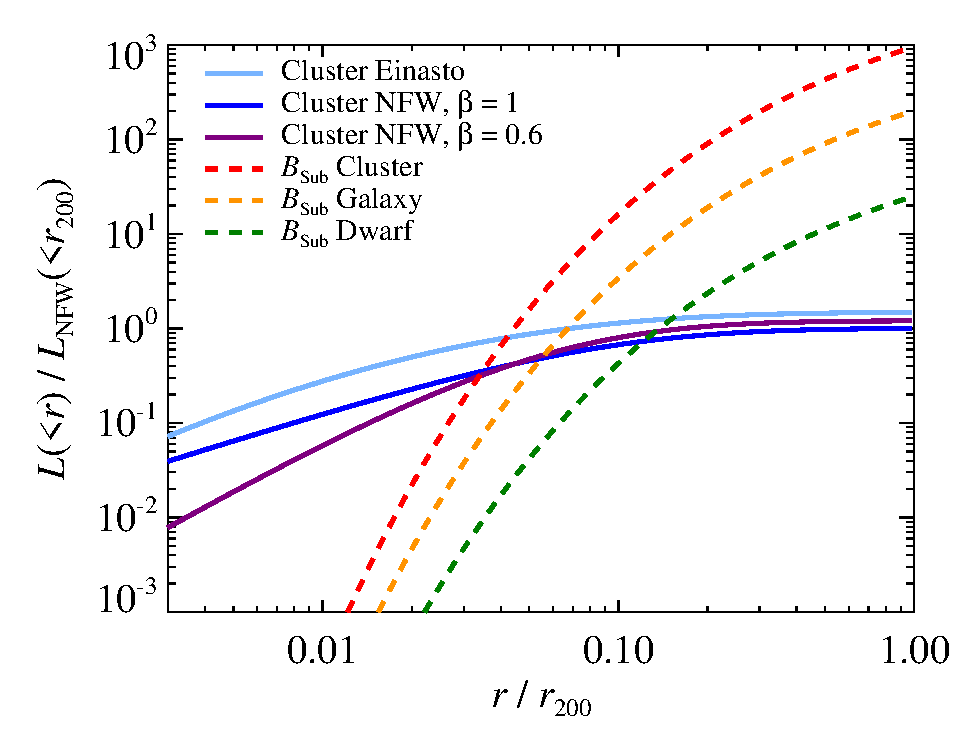
\includegraphics[width=0.99\columnwidth]{figures/dens.prof.eps}
\caption{\it Radial dependence of various luminosity
  contributions. The solid lines show the accumulative smooth
  luminosity from a cluster with the mass $\mvir=10^{15}\,\msun$ for
  three different density profiles; an Einasto profile with
  $\alpha=0.17$ (light blue), a cuspy NFW profile with $\beta=1.0$
  (dark blue), and a core NFW profile with $\beta=0.6$ (purple). The
  dashed lines show the accumulative luminosity from substructures for
  three different mass scales; an $\mvir=10^{15}\,\msun$ galaxy
  cluster (red), an $\mvir=10^{12}\,\msun$ galaxy (orange), and an
  $\mvir=10^{8}\,\msun$ dwarf galaxy (green). All luminosities have
  been normalized with the luminosity within $\rvir$ from a cuspy NFW
  profile. We have assumed the standard value for the limiting
  substructure mass of $M_\rmn{lim}=10^{-6}\,\msun$. Note the large
  expected boost from substructures in clusters ($\sim1000$), and the
  relative small boost in dwarf galaxies ($\sim20$).}
 \label{fig:radial_lum}
\end{figure}

In Fig.~\ref{fig:radial_emis} we show the radius with the maximum
luminosity for substructures and smooth density profiles, both for
three different mass scales. We find that the smooth luminosity per
logaritmic radial bin peaks at $x \dd^2 L/\dd x^2+\dd L/\dd x == 0
\rightarrow r \propto \rvir/3c$. Hence the main contribition to the
luminosity for large mass scales, which are usually assosiated with a
low concentrated DM halos, is focused to the regime around 10\% of
$\rvir$.  It clearly shows how that the main contribution from the
substructures is coming from outer parts of the DM halos, while the
main contribution from the smooth density profiles peaks around the
scale radius. Not that, even though the bulk of substructures have
been erased in the central regions of DM halos, a cluster in
projection has a significant enhancement due to substructures at a
radius of just a few percent of $\rvir$.
\begin{figure}
  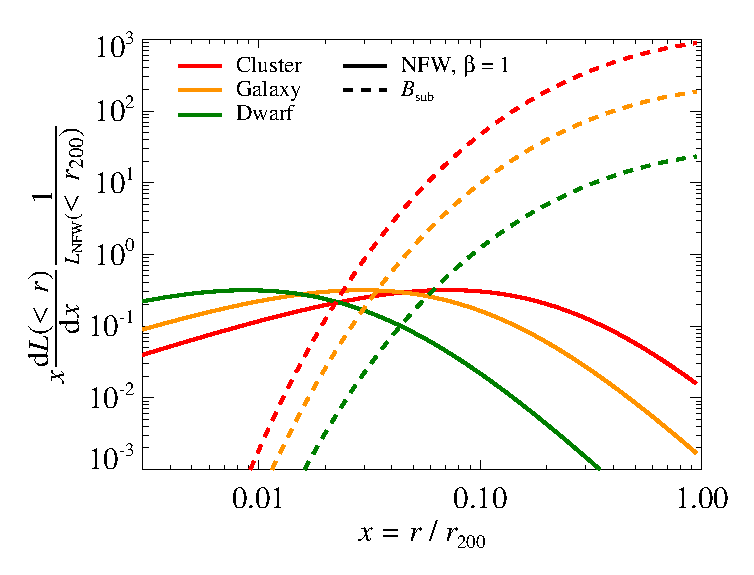
\includegraphics[width=0.99\columnwidth]{figures/emissiv.sub.eps}
  \caption{\it Luminosity dominated radius for different mass
    scales. The solid lines show the emissivity from a cuspy
    $\beta=1.0$ NFW density profile for three different mass scales;
    an $\mvir=10^{15}\,\msun$ galaxy cluster (red), an
    $\mvir=10^{12}\,\msun$ galaxy (orange), and an
    $\mvir=10^{8}\,\msun$ dwarf galaxy (green). The dashed lines show
    the emissivity from substructures for the same three mass
    scales. All emissivities have been normalized with the luminosity
    within $\rvir$ from a cuspy NFW profile. We have assumed the
    standard value for the limiting substructure mass of
    $M_\rmn{lim}=10^{-6}\,\msun$.}
  \label{fig:radial_emis}
\end{figure}


\subsubsection{Cosmic-ray induced gamma-ray emission}
\label{sect:CRs}
On small astrophysical scales, such as supernovae remnants and
galaxies, there are convincing evidences of non-thermal
populations. Especially, in the MW, the cosmic rays are observed
directly as well as indirectly through radio, X-ray, and gamma-ray
emission. On larger scales of the order of few 100~kpc up to Mpc,
there are currently a vast number of observations of radio emission
coming from radio mini halos in the center of cooling flow clusters,
radio relics in the periphery of clusters \cite{2004rcfg.proc..335K}
as well as smooth giant radio halos that have been observed in more
than 50 clusters \cite{2003ASPC..301..143F,2008SSRv..134...93F}. This
type of emission is expected in clusters since the formation process
of a galaxy cluster is a very energetic processes that induces both
turbulence as well as frequently occurring merging and accretion
shocks which both are thought to accelerate large quantities of
relativistic non-thermal protons and radio emitting electrons to high
energies. Thus most of the observed radio emission in clusters is
expected to emerge from cosmic-ray electron induced radio synchrotron
emission. The precise origin of these electrons, in especially relics
and giant radio halos, is still not settled. However, due to the
smoothness of the extended emission and the observed power-law slope
it seems quite natural that they are of hadronic origin. Especially
since the long cooling time of cosmic ray protons (CRps) allows for
both an extended and large population of CRps to build up over the
cluster history \cite{1997ApJ...487..529B}.

When the CRps interact with ambient gas protons, it results in the
production of both charged and neutral pions that decay into
electrons, neutrinos, and gamma-rays. The production of these
secondaries depend both on the gas and CRp densities in the cluster,
where the CRp density roughly trace the gas outside the core regime and
is slightly enhanced in the center. This density scaling implies that
clusters are great targets for Cherenkov telescopes with a high
sensitivity for the central parts of close by clusters. Detecting the
cluster gamma-ray emission is crucial in this respect as it
potentially provides the unique and unambiguous evidence of CRp
populations in clusters through observing the $\pi^0$ bump at about
100~MeV in the spectra. 

We adopt the spectrally and spatially universal gamma-ray model
developed by Pinzke \& Pfrommer \cite{2010MNRAS.409..449P} to estimate
the emission from decaying $\pi^0$:s that dominates over the inverse
Compton emission from primary and secondary electrons above 100~MeV in
clusters. The gamma-ray formalism was derived from high resolution
simulations of clusters of galaxies that included radiative
hydrodynamics, star formation, supernova feedback, and followed CRp
physics using a novel formulation that trace the most important
injection and loss processes self-consistently while accounting for
the CRp pressure in the equation of motion
\cite{2008A&A...481...33J,2007A&A...473...41E,2006MNRAS.367..113P}.
We note that the overall normalization of the CRp and gamma-ray
distribution scales with the maximum acceleration efficiency at
structure formation shock waves. Following recent observations at
supernova remnants \cite{2009Sci...325..719H} as well as theoretical
studies \cite{2005ApJ...620...44K}, we adopt a realistic value of this
parameter and assume that 50\% of the dissipated energy at strong
shocks is injected into CRps while this efficiency rapidly decreases
for weaker shocks \cite{2007A&A...473...41E}.
 

\subsection{Detecting Particle Dark Matter}
\label{sect:PF}
Besides the intrinsic interest in the gamma-ray flux from galaxy
clusters generated by conventional hadronic and electromagnetic
process - which should be close to observability with the Fermi-LAT
data \cite{Berezinsky:1996wx,2007A&A...473...41E,2010MNRAS.409..449P}
- the possible contribution from WIMP dark matter is of greatest
interest. A WIMP (Weakly Interactive Massive Particle) which fulfils
the WMAP bounds on the relic density of cold dark matter (CDM) of
\cite{Komatsu:2010fb}
$$\Omega_{CDM}h^2=0.112\pm 0.0056,$$ will in many cases naturally give
a $\gamma$ yield which may be observable. In addition, there are
possible enhancement effects known, such as the astrophysical boost
from dense substructure of dark matter halos, or the particle physics
boost from the Sommerfeld effect, which may increase the chances of
detection further.

There are three methods for detecting dark matter candidates which are
presently employed: First, at particle physics accelerators such as
CERN's LHC, one is now entering into a new energy regime which may
allow the production of the heavy, electrically neutral and long-lived
particles which may constitute dark matter. From these experiments one
may get the first glimpse of the mass scale beyond the standard model
where dark matter may reside. However, to really show that any of the
hypothetical, new particles created at the LHC is actually the dark
matter, one has to rely on the two other methods available for the
dark matter search, namely direct and indirect detection. Direct
detection methods, which are presently evolving rapidly use the feeble
interaction between that dark matter particles of the galactic halo
and nuclei such as Germanium, Sodium, Iodine, Argon or Xenon to infer
the scattering cross section and a rough estimate of the mass of the
dark matter particle (for the currently most sensitive search, see
\cite{Aprile:2010um}). A characteristic of this method is that it
basically only depends on the local dark matter density (which is
rather well determined to be around $0.4$ GeV/cm$^3$) and the basic
cross section for dark matter - nucleus scattering. A disadvantage is
that it does benefit from the two enhancement mechanisms mentioned
above, boost from substructure and/or the Sommerfeld effect. Also, it
cannot be excluded - although it seems at present improbable - that
the local halo structure is such that the solar system happens to be
in an underdense region.

In indirect detection, on the other hand, in particular in the photon
channel, one searches for products of dark matter annihilation in the
galactic halo and beyond. Particularly interesting targets are the
galactic center (for a recent possible indication of a signal, see
\cite{Hooper:2010mq}), the dwarf galaxies surrounding the Milky Way
\cite{Strigari:2006rd,Essig:2009jx,2010JCAP...01..031S}, galaxy
clusters (the focus of this work)
\cite{Ghigna:1998vn,Lewis:2002mfa,Boyarsky:2006kc,2006A&A...455...21C,2009PhRvL.103r1302P},
and even the cosmological large scale structure
\cite{Bergstrom:2001jj,Ullio:2002pj,Taylor:2002zd,Elsaesser:2004ap,Cuoco:2010jb,Abazajian:2010sq,Abdo:2010dk,Zavala:2011tt}.

There is also a possiblity to search for dark matter annihilation
indirectly in antimatter channels, like antiprotons or positrons. Here
diffusion is, however, very efficient which means that the directional
signature which is so important for gamma-rays, is completely
erased. This method has, however, recently been much in focus due to
the surprising rise with energy of the electron to proton ratio
measured by the PAMELA satellite experiment \cite{Adriani:2008zr} and
the ``bump'' in the total electron plus positron spectrum detected by
Fermi \cite{Abdo:2009zk}. The viable particle physics models
describing these results contain some non-trivial, or even unnatural
elements, however. First of all, annhilation to quarks has to be very
much suppressed, due to the non-observation of an enhanced antiproton
flux by PAMELA \cite{Adriani:2010rc}. This means that only so-called
{\em leptophilic} models, where the annihilation only goes to leptons
have to be considered. Here, one has to have a sizeable fraction going
to muons and tau leptons, as the shape of the spectrum disfavours
direct annihilation into electrons and positrons. To get agreement
with the measured absolute rates, one also has to have a large boost
factor (of the order of at least several hundred), which is difficult
to achieve with substrucutre alone. An additional enhancement of the
annihilation rate has to be invoked, for example given by the {\em
  Sommerfeld effect}. This basically means that the usual connection
between annihilation rate at decoupling (when relative velocities $v$
were of order $0.2 - 0.3$), which gives the relic density, and
present-day annihilation in the halo (with velocities $v\sim 10^{-3}$)
is broken. This would come about because the dark matter sector
contains additional light particles which mediates an interaction with
almost bound states which enhance the wave function at the relative
origin, and therefore the annihilation rate (for a pedagogical review
of viable scenarios, see \cite{ArkaniHamed:2008qn}). As a final
difficulty of these models, the lack of an inverse-compton signature
from the galactic center means that only shallow density profiles can
describe the galactic dark matter density distribution
\cite{Bertone:2008xr,Cirelli:2008pk,Bergstrom:2008ag}. (For a review
of the dark matter modelling of these effects, see
\cite{Bergstrom:2009ib}. For a recent treatment, showing still viable
models, see \cite{Finkbeiner:2010sm}.)

A more standard explanation of the PAMELA/Fermi excess would be
pulsars or other supernova remnants (e.g.,
\cite{Hooper:2008kg,Ahlers:2009ae}). In that case, dark matter would
more likely be explained by the standard scenario of a WIMP, for
example the thoroughly studied lightest supersymmertric neutralino
(for reviews, see
\cite{Jungman:1995df,Bergstrom:2000pn,Bertone:2004pz}). We note that
the soon to be launched AMS-02 experiment on the International Space
Station \cite{ams02} may gave interesting clues to the origin of the
antimatter excess.

\subsubsection{Leptophilic models}
\label{sect:LP}
The results of PAMELA \cite{Adriani:2008zr} and Fermi-LAT
\cite{Abdo:2009zk} (and to some extent ATIC
\cite{2008Natur.456..362C}, although the bump seen there at 600 GeV
has not been reproduced by other experiments) has caused intense
activity in the theoretical dark matter community. At first, there was
skepticism whether such a large signal could be compatible with a
WIMP. However, the possibility of an enhanced annihilation rate due to
dark matter halo substructure has been realised for a long time
\cite{1993ApJ...411..439S,Bergstrom:1998zs,Moore:1999nt}, although it
is difficult to achieive the boost factor of the order of a few
hundred to a thousand in the solar neighbourhood, as substructure
according to numerical simulations is most important in the outer
portions of the halo, due to tidal stripping of subhaloes in the inner
part. Another potentially very important effect which may explain the
large boost had been found a few years earlier, namely the Sommerfeld
enhancement. This effect, was computed for electromagnetism by Arnold
Sommerfeld may years ago \cite{sommerfeld} and recently rediscovered
in the quantum field theory of dark matter
\cite{2005PhRvD..71f3528H,2007NuPhB.787..152C,2009PhRvD..79a5014A}.
In quantum mechanics describing electron scattering and electron
positron annihilation, it is caused by the distortion of the plane
wave describing the relative motion of the annihilating particle pair,
due to the near formation of a bound state caused by photon
exchange. In the ladder approximation for QED, one reproduces the
Sommerfeld effect, and the square of the relative wave function at the
origin (which enters into the probablity for the short-distance
process of annihilation) is increased by the factor
\cite{2009PhRvD..79a5014A}
$$
S_{QED}=\frac{|\psi(0)|^2}{|\psi^{(0)}(0)|^2}=|\frac{\frac{\pi\alpha}{v}}{1-e^{-\frac{\pi\alpha}{v}}}|,
$$ with $\alpha =e^2/\hbar c$ the fine-structure constant, and $v$ the
realtive velocity. This amounts to $S_{QED}=\pi\alpha/v$ for small
velocities. For a Yukawa-like particle of mass $m_\phi$, mediating a
weak attractive force with coupling contant $\alpha_Y$ between dark
matter particles $\chi$ with mass $m_\chi$, the small-velocity limit
of the enhancement becomes instead
$$
S_Y\sim\frac{\alpha_Y m_\chi}{m_\phi}.
$$ In the general case, with mediators that may also excite virtual
charged particles in the dark matter sector, one has to solve
numerically a coupled system of differential equations using
appropriate boundary conditions
\cite{2005PhRvD..71f3528H,2007NuPhB.787..152C,2009PhRvD..79a5014A}. In
some cases, the enhancement factor $S$ can be as high as several
hundred to a few thousand, depnding however on the exact parameters of
the theory. The effect is usually strongly velocity-dependent,
depending on velicity as $1/v$ or, in the fine-tuning case of being
very near resonance, as $1/v^2$. This means that in a virialised
system (such a a galaxy cluster) with large velocity dispersion
$v_{\rm cl}$ the Sommerfeld enhancement will be smaller than the one
expected in a single galaxy such as the Milky Way, roughly by a factor
$v_{\rm MW}/v_{\rm cl}$.


As leptophilic models, apart from being slightly contrived from the
particle physics point of view, are also rather limited by several
sets of astrophysical data, we take advantage of the recent reanalysis
\cite{Finkbeiner:2010sm} to define a benchmark leptophilic model that
is still viable.  It is found that the bounds from WMAP5 approximately
imply a Sommerfeld boost factor $S$ which has to satisfy $S(v\to
0)\lesssim 200/f\ (m_Y/1$ GeV$)$, where $f$ is the fraction of energy
from dark matter annihilation that ionizes the intergalactic medium,
$f\sim 0.7$ for annihilation to electrons and a factor a a few smaller
for all other standard model final states.

Taking into account the whole cosmic history of leptophilic models,
also utilizing limit on spectral and polarization distorsions of the
CMB, the maximal value for the boost factor for a 1 to 2 TeV particle
and sub-GeV force carriers is found to be \cite{Finkbeiner:2010sm}
between 400 and 800. Although lower than the first estimates (e.g.,
\cite{Bergstrom:2009fa,Meade:2009iu}) this is still enough to explain
the PAMELA and Fermi excess, given other astrophysical uncertainties.

To connect easily to our previous work \cite{2009PhRvL.103r1302P}, we
choose as our benchmark leptophilic model one with mass $1.6$ TeV and
Sommerfeld boost $S=300$.

\subsubsection{Supersymetric dark matter}
The most studied models for dark matter are supersymmetric ones,
especially models where the lightest supersymmetric particle, in most
models the lightest neutralino, is stable. The stability is assured in
viable SUSY models due to a discrete symmetry, $R$-parity. This
symmetry is needed from the particle physics point of view to avoid
fast proton decay, and automatically makes the lightest supersymmetric
particle stable, and therefore a good candidate for dark matter. In
addition, as the coupling to ordinary matter is given by gauge
couplings, the neutralino is automatically a WIMP
candidate. Unfortunately, the breaking of supersymmetry (which has to
be there since otherwise, e.g., there would exist a scalar electron
with the same mass as the electron) means that a large number of
essentially free parameters enter actual calculations.  The neutralino
is then a linear combination of the supersymmetric partners of the
U(1) gauge boson, one of the SU(2) gauge bosons, and the two Higgs
doublets in the Minimal Supersymmetric extension of the Standard Model
(the MSSM) with mixing coefficients which depend on the SUSY breaking
parameters \cite{1984NuPhB.238..453E}. The parameter space is very
large, too large in general to scan efficiently even with the most
powerful computers. Therefore, often simplifying assumptions are made
to limit the number of free parameters. Even then, a large number of
viable models is found which give a relic density consistent with the
WMAP data. This means that they are indeed very good templates for
WIMP dark matter, something that explains their popularity besides the
subjective statement that few more plausible models for dark matter
have been put forward so far.

The the wave function of the lightest neutralino can be written
$$
\tilde\chi_1=a_1\tilde B+a_2\tilde W_3+a_3 \tilde H_1^0+a_4\tilde H_2^0,
$$
with 
$$
\sum_{i=1}^4 |a_i|^2=1.
$$
the gaugino fraction of a given neutralino is $|a_1|^2+|a_2|^2$ whereas $|a_3|^2+|a_4|^2$ is the higgsino fraction. 


We use the \ds package \cite{ds} to compute the mass, couplings and
relic density for a given set of parameters.  Actually, we take
advantage of so-called benchmark models, which have been proposed in
different contexts (in particular in \cite{Bringmann:2008kj} giving
predictions for the MAGIC experiment), and which give a good
representation of models with high enough gamma-ray rates to become
the first candidates for dark matter indirect detection in imaging air
Cherenkov telescopes. We use the following supersymmetric benchmark
models:

\begin{itemize}
\item
 $I′$: This model was introduced in \cite{2004EPJC...33..273B}, where
  its phenomenology at colliders was studied. Annihilation directly
  into lepton pairs is suppressed for neutralinos due to their
  Majorana nature and therefore helicity suppression for annihilation
  in the galactic halo \cite{1983PhRvL..50.1419G}. The higher order
  process (inner bremsstrahlung, IB) $\tilde\chi_1\tilde\chi_1\to
  \ell^+\ell^-\gamma$, which does not suffer from helicity suppression
  \cite{1989PhLB..225..372B,2008JHEP...01..049B}, gives a considerable
  contribution due to light sleptons in this model.

\item $J′$: This model, also from \cite{2004EPJC...33..273B} is in the
  so-called coannihilation tail. The sleptons are nearly degenerate
  with the neutralino, which causes the large IB from the leptonic
  final states to give a high enhancement of the flux.

\item $K′$: A representative model for the funnel region, where the
  annihilation dominantly occurs in the $s$-channel through exchange
  of the pseudoscalar Higgs boson \cite{2004EPJC...33..273B}. Here IB
  contributions are not important.

\item $J^*$: Annihilation in the so-called coannihilation region,
  introduced in \cite{2008JHEP...01..049B} as BM3, with a particularly
  large IB contribution.

\end{itemize}



\subsubsection{Final state radiation}
There are two types of radiative processes which are important for our
benchmark models, first the usual QED final state radiation (FSR) for
both the leptophilic model and for supersymmetric models with charged
final states. In addition, there may be direct emission from a
virtual, charged, exchanged particle (such as a spin-0 slepton or
squark), internal bremsstrahlung, IB. The latter is essentially only
important when there is a helicity suppression for the lowest order
annihilation process, which is the case for neutralinos, whose
Majorana nature make the annihilation rate in the $s$ wave
proportional to $m_f^2$, for final state fermion $f$. Interestingly,
both the gamma-ray and fermion energy spectra are peaked at the
highest energy for this process, which can in some models cause a
rather spectacular bump in the spectra for these models.

The photon spectrum resulting from FSR is universal with only a
weak dependence of the underlying particle physics model. The photon
yield from this process is given by (see
e.g. \cite{2008JHEP...01..049B})
\begin{equation}
\frac{\dd N_{X \bar{X}}}{\dd x} \approx \frac{\alpha Q_X^2}{\pi}
\mathcal{F}_X(x) \log\left[\frac{4 m_\chi^2\left(1-x\right)}{m_X^2}\right]\,.
\end{equation}
Here, the normalized photon energy $x=\eg/m_\chi c^2$, 
$\alpha =e^2/\hbar c$ is the fine-structure constant, 
$Q_X^2$ and $m_X$ the
charge and mass of the particle $X$, respectively. The function
$\mathcal{F}_X(x)$ depends on the spin of the final state and is given
by
\begin{equation}
\mathcal{F}_\rmn{fermion}(x) = \frac{1+\left(1-x\right)^2}{x}\,
\end{equation}
for fermions. 

The differential energy spectrum for the IB process is more
complicated (see \cite{1989PhLB..225..372B,2008JHEP...01..049B}), but
can be computed using {\sc DarkSUSY}. The differential photon energy
spectra for all our benchmark models are shown in
Fig.~\ref{fig:bmspectra}.  The peaking at high photon energy and the
resulting bump caused by inner bremsstrahlung is clearly seen for
benchmark models $I´$, $J´$, and $J^*$.


\subsection{Radiative processes}
In this section we outline the basics of inverse Compton (IC)
emission. As target radiation fields we consider both cosmic microwave
background (CMB) photons, and the light from stars and dust (SD). We
derive a semi-analytic model from which we can estimate the spectral
and spatial distributions of SD as a simple function of cluster mass.

\subsubsection{Inverse Compton}
\label{sect:IC}
The standard IC source function is given by
\cite{1979rpa..book.....R}:
\begin{eqnarray}
  q_{\rmn IC}(\eg, r) &=&  \frac{\dd^3 N_\gamma}{\dd V\,\dd t\,\dd \eg} = 
 \frac{3}{4}c\,\sigma_\rmn{T}
\int\dd \eph \frac{n_\rmn{ph}(\eph)}{\eph}\nonumber\\
&\times& \int \dd \ee\,\frac{\dd n_\e}{\dd \ee}(\ee,r)\,
 \frac{\left(m_\e c^2\right)^2}{\ee^2}G(\Gamma_\e,q)\,,\nonumber\\
  \label{eq:ICemiss}
\end{eqnarray}
where $\ee$ is the energy of the upscattering electrons and $\eph$ is
the energy of the background photon field. We represent the Thomson
cross-section with $\sigma_\rmn{T}$ and the full differential
Klein-Nishina (KN) cross-section is captured by
\cite{1970RvMP...42..237B}:
\begin{equation}
\label{eq:KN_spec}
G(\Gamma_\e,q) = 2q\ln{q}+(1+2q)(1-q)+ 
\frac{1}{2}\frac{\left(\Gamma_\e q\right)^2\left(1-q\right)}
     {1+\Gamma_\e q}\,,
\end{equation}
where
\begin{equation}
\Gamma_\e=\frac{4\eph \ee}{\left(m_\e c^2\right)^2}\,,\qquad \rmn{and} \qquad  
q=\frac{\eg}{\Gamma_\e\left(\ee-\eg\right)}\,.
\end{equation}
The full KN cross-section accounts for the less efficient energy
transfer between the photon and electron and results in a steepening
of the IC gamma-ray spectrum. In the low energy Thomson regime the IC
spectrum $F_\gamma\sim E_\gamma^{-(\alpha_\e-1)/2}$, however when
$\Gamma_\e \gg 1$ the IC spectrum steepens due to the KN suppression
to $\eg^{-\alpha_\e}\log(\eg)$. Here we denote the steady
state electron spectrum by $\alpha_\e$.

We account for two major contributions to the number density of
radiative background fields $n_\ph$; the CMB photons and the infra-red
(IR) to ultra-violet (UV) light emitted by SD. The number density for
the SD is given by $n_\ph\equiv\frac{\dd^2 N_\ph}{\dd V \,\dd
  \eph}(\eph,r)= \frac{u_\sd(\eph,r)}{\eph^2}$ where the SD energy
density $u_\sd(\eph,r)$ is given in Eq.~(\ref{eq:U_SD}). We model the
CMB photon spectrum as a photon gas that is isotropically distributed
and follows a black body spectrum with the temperature $T=2.73\,$~K:
\begin{equation}
\label{eq:photon_gas}
  n_\rmn{ph}(\eph) = \frac{\dd^2 N_\ph}{\dd V \,\dd \eph} =
  \frac{1}{\pi^2(\hbar c)^3}\frac{\eph^2}{\exp(\eph/k_\B T)-1}\,.
\end{equation}
Note that the typical energy of a black body photon before scattering
is given by $<\eph>=\epsilon_\ph/\tilde{n}_\ph\approx\,2.70 k_\B T$,
where $\tilde{n}_\ph$ and $\epsilon_\ph$ are the number- and
energy-density derived by integrating $n_\ph(\eph)$ and $\eph
n_\ph(\eph)$ over the photon energy $\eph$, respectively.

The electrons injected from annihilating DM also suffer from diffusive
and radiative losses. Hence we have to calculate the equilibrium
spectrum of the electrons plus positrons denoted by $\frac{\dd
  n_\e}{\dd \ee}$ in Eq.~(\ref{eq:ICemiss}). We derive this stationary
solution using the CR transport equation (neglecting convection and
re-acceleration effects):
\begin{eqnarray}
\label{eq:CRdiffusion}
\frac{\partial}{\partial t}\left(\frac{\dd n_\e}{\dd \ee}\right) = 
&\nabla& \left[D\left(\ee,\bx\right)\nabla\frac{\dd n_\e}{\dd \ee}\right] + 
\frac{\partial}{\partial \ee}
\left[b\left(\ee,\bx\right) \frac{\dd n_\e}{\dd \ee}\right]
 \nonumber \\
&+& q_\e(\ee,\bx)\,,
\end{eqnarray}
where $D(\ee,\bx)$ denotes the diffusion coefficient and $b(\ee,\bx)$
the energy loss term. The source function $q_\e(\ee,\bx)$ yields the
number of electrons and positrons produced per unit time, energy and
volume element at the position $\bx$:
\begin{equation}
q_\e(\ee,r)=\sum_f\frac{\dd N_{\e,f}}{\dd \ee}(\ee) B_f \Gamma_f(r) \,,
\end{equation}
where the annihilation rate density $\Gamma_f(r)$ is defined in
Eq.~(\ref{eq:ann_rate}). The sum runs over the kinematically allowed
annihilation final states $f$, each with a branching ratio $B_f$ and a
differential spectrum $\frac{\dd N_\e^f}{\dd \ee}$ that represents the
number of electrons plus positrons resulting from an annihilation
event. For neutralinos annihilating directly into electrons and
positrons we model the spectral distribution with $\frac{\dd
  N_\e^f}{\dd \ee}= 2\delta(\ee-m_\chi c^2)$. We use DarkSUSY to
compute both the spectra when neutralinos annihilate directly into a
$\mu^+$ and $\mu^-$ in the leptophilic model as well as in the four BM
models where a fraction of the annihilating neutralinos is converted
into electrons and positrons (see Sect.~\ref{sect:PF} and
Fig.~\ref{fig:q_DM} for further details).
%(see \cite{2009JCAP...01..016B} and references therein,
%also see fit).  

The electrons and positrons loose their energy on a timescale that is
shorter than the diffusive timescale in the ICM of galaxy clusters for
CR electrons with $\ee \gtrsim\,$~MeV (CHECK). Hence, we neglect the
first term of the r.h.s. in Eq.~(\ref{eq:CRdiffusion}), and derive an
expression for the equilibrium number density:
\begin{eqnarray}
{\frac{\dd n_\e}{\dd \ee}}\left(\ee, r \right) &=&
 \frac{1}{b(\ee, r)} \int_{\ee}^{\mx c^2} \dd \ee' \, 
  Q(\ee', r),
\label{eq:nds}\\
b(\ee,r) &=& \tilde{b}
\left[\frac{B^2_{\rm CMB}}{8\pi}+\frac{B^2(r)}{8\pi}+u_\sd(r)\right] \ee^2\,,
\\\tilde{b}&=&\frac{4\sigma_{\rm T}c}{3(m_{\rm e}c^2)^2}\,.
\end{eqnarray}
Here we include the three main radiative loss processes for the CR
electrons and positrons: (1) IC losses on CMB photons where the
equivalent field strength of the CMB is denoted by $B_{\rm
  CMB}=3.24\mu\rmn{G}$. (2) Synchrotron losses on ambient
magnetic fields where we parameterize the magnetic field in the galaxy
cluster by $B(r) = 3\mu\rmn{G} \,[n_{\rm e}(r)/n_{\rm
    e}(0)]^{\alpha_\B}$, which follows from flux frozen magnetic
fields. We adopt a magnetic decline of $\alpha_\B=0.7$ in this
work. (3) IC losses on starlight and dust with an energy density
$u_\sd(r)$ given by Eq.~(\ref{eq:U_SD}), which we derive in the
following subsection.

{\it IC -- dust and starlight}\\ Galaxy clusters are typically
characterized by the hot gas in the ICM and the collection of
gravitationally bound galaxies. The emission in the IR and UV
wavelengths emerge from dust and starlight in both the galaxies and
the ICM (e.g. \cite{2006ApJ...648L..29P} and
\cite{2009MNRAS.399.1694G}). Much of the radiation leaks out from the
galaxy into the ICM, which give rise to similar spectral distributions
for the galaxies and the ICM in these wavelengths. Hence, we use the
accurately measured light from galactic dust and starlight for the ISM
to model the ICM. We characterize the spectra through a fit to the
galactic spectra presented in \cite{2006ApJ...648L..29P}. The spatial
distribution of the SD light in clusters is extracted from a stacked
emission analysis of Sloan Digital Sky Survey (SDSS) data at the
redshift $\sim 0.25$ \cite{2005MNRAS.358..949Z}. Finally, we fix the
normalization for the light from stars and dust individually in a
galaxy cluster using using the IR to X-ray luminosity scaling relation
found in \cite{2008A&A...490..547G}. The X-ray luminosities for the
clusters used in this work are listed in the extended HIghest X-ray
FLUx Galaxy Cluster Sample (HIFLUGCS) \cite{2002ApJ...567..716R} from
the Rosat all-sky survey. Note that we have added the Virgo cluster to
the sample that we nevertheless refer to as extended HIFLUGCS
catalogue in the following.

\begin{figure}%[t]
 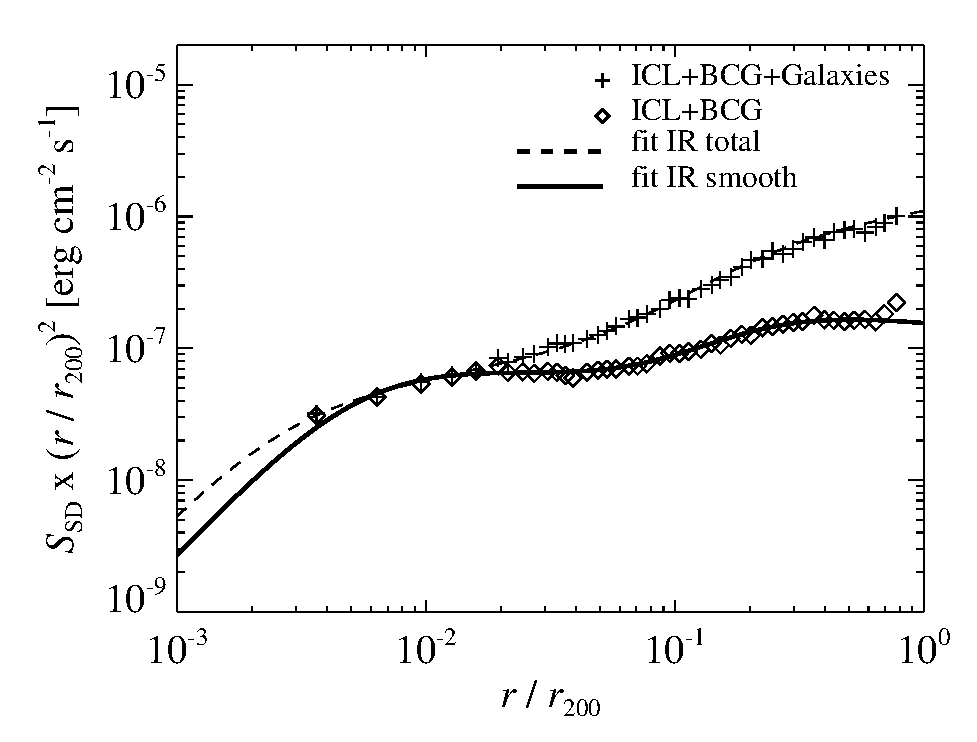
\includegraphics[width=0.99\columnwidth]{figures/SB.photon.eps}
\caption{\it Spatial dependence of light from stars and dust. We show
  2D surface brightness profiles in the $r$-band ($\sim 1\,\ev$)
  obtained from stacked clusters in the Sloan Digital Sky Survey
  (SDSS) at the redshift $z \sim 0.25$ \cite{2005MNRAS.358..949Z}. The
  brightness profiles have been weighted with the $\rvir$ normalized
  area inside radius $r$, and trace the radial dependence of the
  luminosity from stars and galaxies. The crosses show the total
  observed starlight including the diffuse intracluster (ICL), the
  galaxies, and the brightest cluster galaxy (BCG) in the center of
  the cluster. The diamonds denote the observed starlight from the
  ICL and the BCG. The solid line show the fit to the data of the
  total light including the ICL, the BCG, and the galaxies, while the
  smooth component is represented by the dashed line that is fitted to
  only the ICL and the BCG.}
 \label{fig:SD_spatial}
\end{figure}
\begin{figure}%[t]
 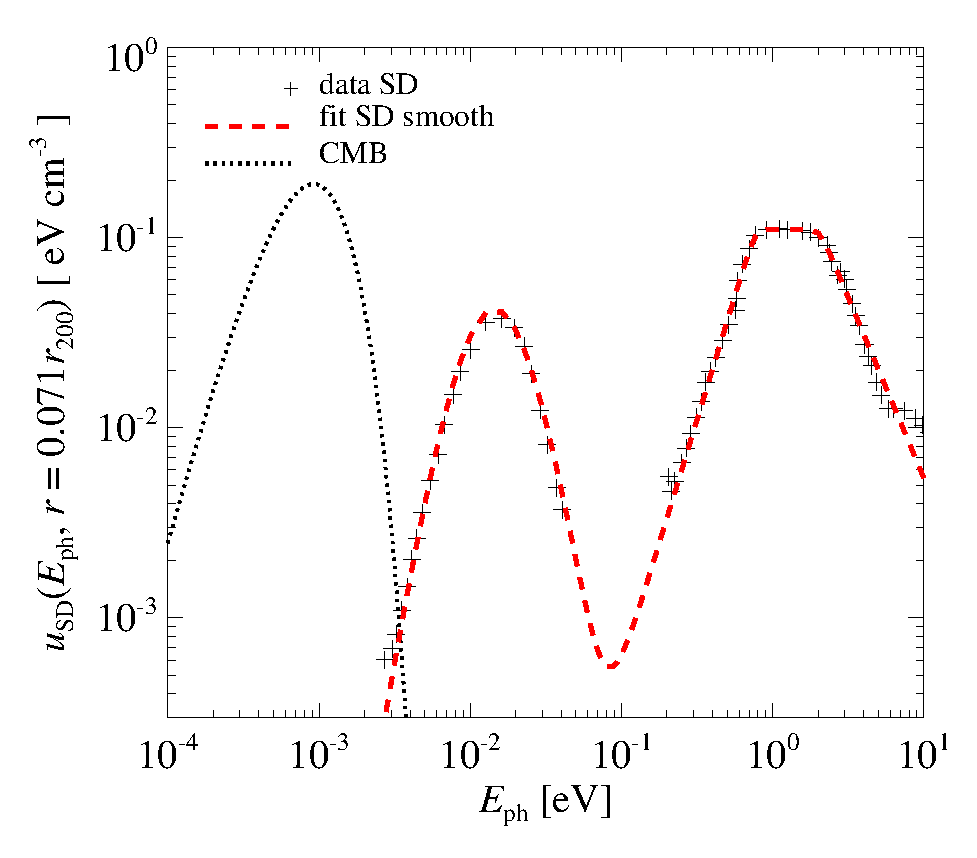
\includegraphics[width=0.99\columnwidth]{figures/fit.porter.v2.eps}
\caption{\it Spectral dependence of radiation fields in a cluster of
  galaxies. The black dotted line in the left peak show the spectrum
  of CMB photons using a black body with a temperature of
  $2.73$~K. The crosses in the middle and right peaks represent the
  measured spectra from stars and dust (SD), respectively, and are
  derived in \cite{2006ApJ...648L..29P} for a galaxy. We normalize the
  individual SD spectrum separately using the observed luminosity from
  SD in clusters. The SD luminosity is related to the cluster mass
  through Eq, where we use have used the mass
  $\mvir=4.0\times10^{13}\msun$ in this figure. Finally we renormalize
  the SD spectra to the radius $r=0.071\rvir$, where the smooth energy
  density of the SD light (see Fig.~\ref{fig:SD_Edens}) equals the
  energy density of the CMB. The red dashed lines show the fitted SD
  spectral model.}
 \label{fig:SD_spectra}
\end{figure}
\begin{figure}%[t]
 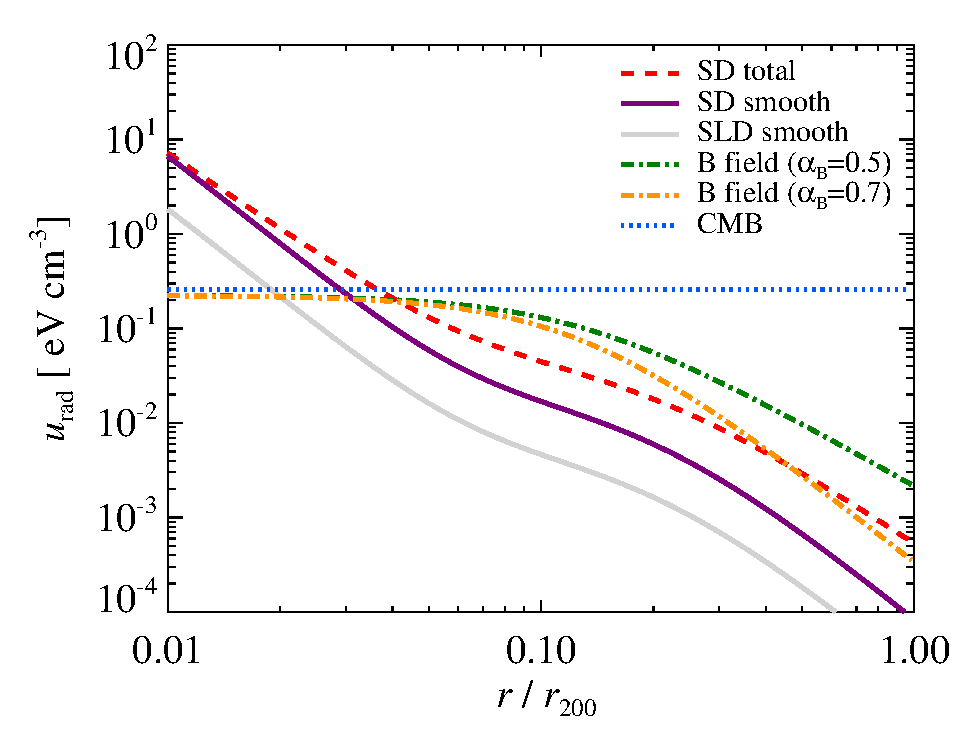
\includegraphics[width=0.99\columnwidth]{figures/ucool.eps}
 \caption{\it Spatial dependence of the energy density of radiation
   fields in a cluster of galaxies. The energy density of the CMB,
   shown by the blue dotted line, is isotropic throughout the cluster,
   hence represented by a flat profile with
   $u_\rmn{cmb}=0.26\,\rmn{eV}\,\rmn{cm}^{-3}$. The energy density of
   the light from stars and dust (SD) is denoted by the red dashed
   line and the solid purple line for the total SD light and the
   smooth SD light, respectively. The SD light has been renormalized
   to a cluster with the mass $\mvir=4.0\times10^{13}\msun$. Finally we
   show the energy density two magnetic field models with a central
   magnetic field of 3~$\mu G$. The magnetic field scales with the gas
   density to the power $\alpha_\rmn{B}$; green dash-dotted line
   ($\alpha_\rmn{B}=0.5$) and orange dash-dotted line
   ($\alpha_\rmn{B}=0.7$). Note that the SD radiation is dominating
   the energy density inside $\sim0.1\,\rvir$.}
 \label{fig:SD_Edens}
\end{figure}

\section{Spectral gamma-ray distribution}
\label{sect:spectral}
Spectrally resolved indirect DM searches have the advantage of probing
different DM models through their characteristic spectral
distributions. To make current and future DM searches more effective
it is important to know in which energy band to focus the efforts in
order to maximize potential DM signal over expected background.

We dedicate this section to the spectral distribution of gamma-ray
flux from clusters. The flux emerge from a leptophilic DM model that
emit final state radiation and give rise to substantial amounts of
electrons and positrons that IC upscatter background radiation fields
to high energies. We also consider a few supersymmetric DM models with
a high gamma-ray yield in the form of continuum emission and IC
induced emission. In addition to the annihilating DM, we estimate the
gamma-ray flux induced by shock accelerated CRps.

In Fig.~\ref{fig:diff_BM} we show the differential flux from the
Fornax cluster which is one of the best clusters for indirect DM
searches due to its relative high DM induced fluxes and low CR induced
fluxes. We derive the emission from four different supersymmetric BM
models and compare the flux to both the emission induced by CRps as
well as to the differential gamma-ray upper limits set by Fermi-LAT
after 18 months of observations \cite{2010ApJ...717L..71A}. We find
that the upper limits are not violated, although the predicted DM flux
that is dominated by the continuum emission from $\Kp$ and $\Ip$
models (shown in the left panels) are close to the upper limits and
can potentially be probed by the Fermi 3 year data. Furthermore, the
expected masking gamma-ray signal induced by CRps is about a factor 10
below the DM continuum flux from the $\Kp$ and $\Ip$ BM models around
10~GeV. However, the IC emission from upscattered CMB and SD photons
is at least a factor 10 lower than the expected flux from CRps above
100~MeV, making it very hard to distinguish such a signal from the
foreground due to the similar spectral index. For energies below
100~MeV we expect shock accelerated electrons and positrons to be
dominating \cite{2010MNRAS.409..449P} over the supersymmetric DM
induced leptons. Hence the IC emission from supersymmetric DM in
clusters can for most applications safely be neglected compared to the
CRps and DM continuum emission.

\begin{figure*}
\begin{minipage}{2.0\columnwidth}
 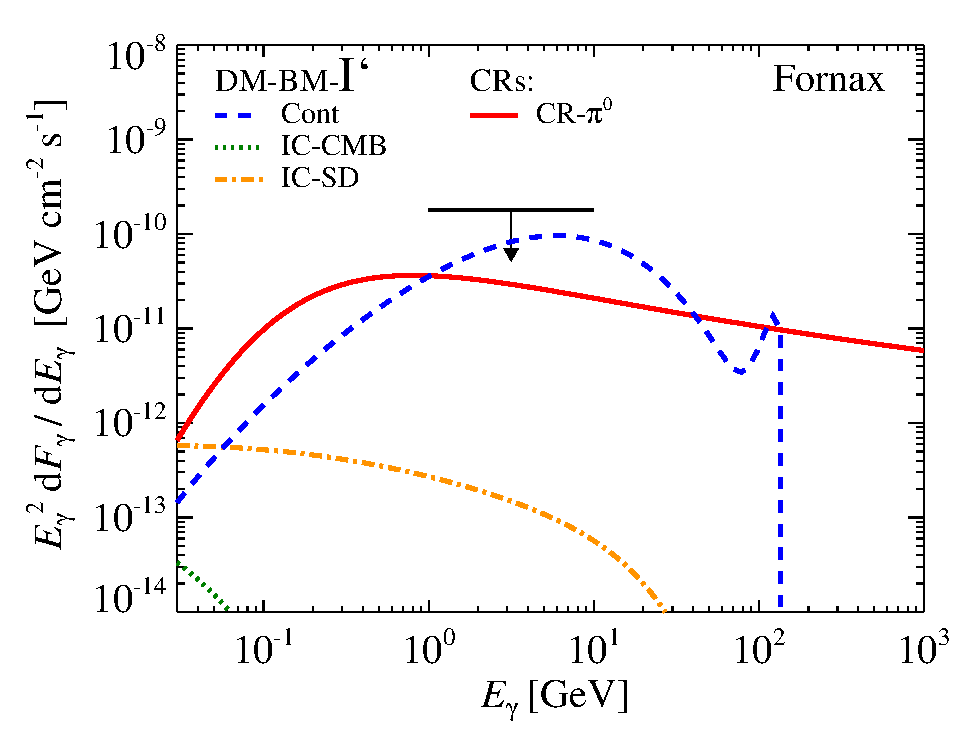
\includegraphics[width=0.49\columnwidth]{figures/flux.BMcompI.v9.0.1deg.1.6T.SubMass.IR2.noMW.woGal.eps}
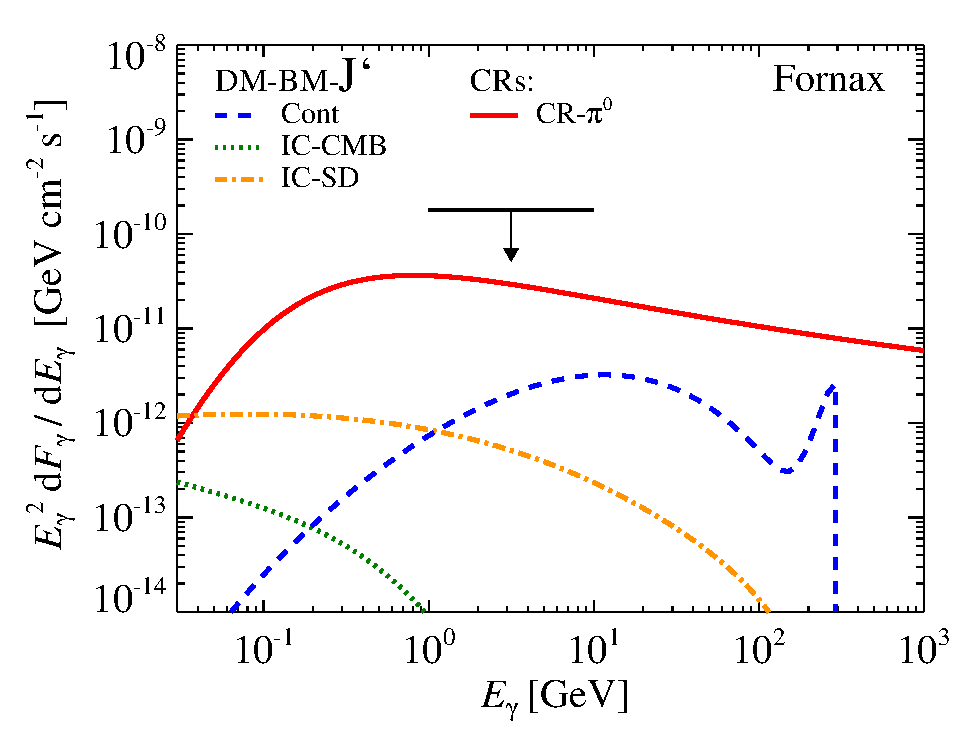
\includegraphics[width=0.49\columnwidth]{figures/flux.BMcompJ.v9.0.1deg.1.6T.SubMass.IR2.noMW.woGal.eps}
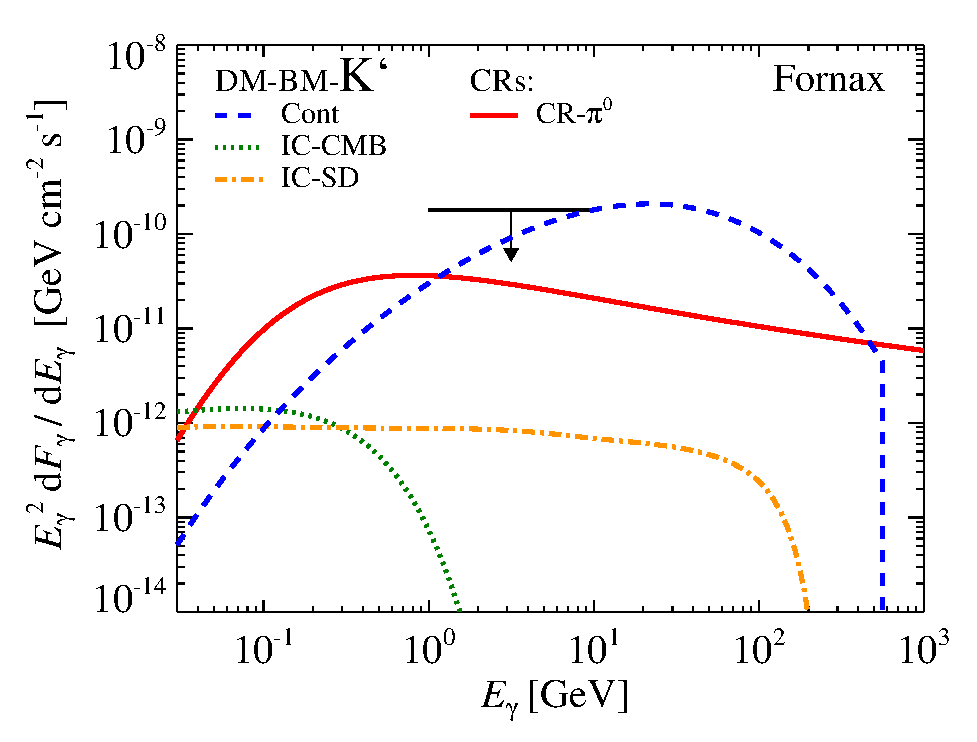
\includegraphics[width=0.49\columnwidth]{figures/flux.BMcompK.v9.0.1deg.1.6T.SubMass.IR2.noMW.woGal.eps}
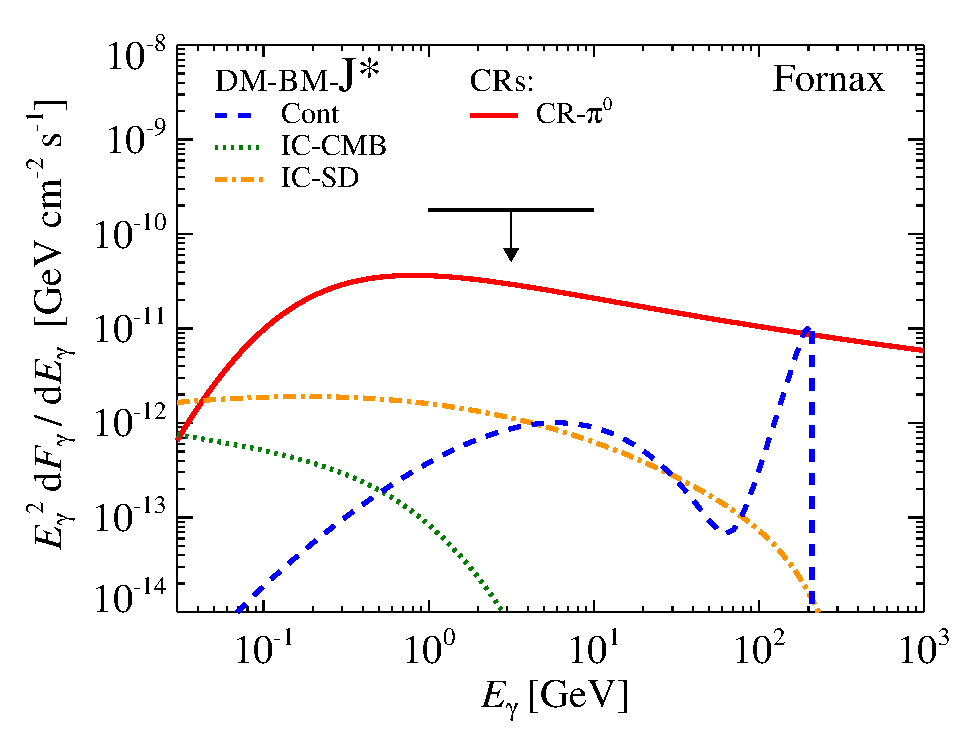
\includegraphics[width=0.49\columnwidth]{figures/flux.BMcompJs.v9.0.1deg.1.6T.SubMass.IR2.noMW.woGal.eps}
\caption{\it Comparing the differential flux from different models: we
  show the continuum emission from DM benchmark (BM) models (blue
  dashed), electrons and positrons from DM BM models that inverse
  Compton upscattered both CMB photons (orange dash-dotted) as well as
  dust and star photons (green dotted), and CRp induced gamma-ray
  emission (red solid). Each panel is associated with an individual DM
  BM model; upper left $\Ip$, lower left $\Kp$, upper right $\Jp$, and
  lower right $\Js$. The emission is calculated for the Fornax cluster
  using a point spread function of $0.1\deg$ and a boost from
  substructures of 570. We find bright prospects for detecting the
  continuum emission that is dominating the total emission in the GeV
  energy range. Also note that, above 100~MeV the total inverse
  Compton emission is at least a factor 10 smaller than the emission
  expected from both the continuum emission and the emission coming
  from CRps.}
 \label{fig:diff_BM}
\end{minipage}
\end{figure*}

\del{CONSIDER REWRITING, START WITH PHYSICS, THEN DISCUSS DOMINATING
CONTRIBUTIONS, PEAKS, AND SPECTRAL INDICES}

In Fig.~\ref{fig:IR_comp} we show the total IC emission as well as its
individual contributions from different IC upscattered radiation
fields. The left panel show the gamma-ray emission from the LP model
and the right panel from the $\Kp$ BM model, and for comparison we
overplot the emission expected from the CRps. Due to the flat electron
and positron spectrum resulting from the LP DM model and the smaller
mean energy of the CMB compared to the SD, we find that the
upscattered CMB photons dominate the total DM IC emission in the
energy regime below 100~GeV, while the SD dominate above this
energy. For the BM models this transition is shifted towards a smaller
energy since the electron and positron spectrum has a steep spectral
distribution that suppresses low energy photon fields. This
suppression is also seen in the relative normalization of the flux
where the IC from both CMB and dust photons are lower compared to the
starlight simply because the starlight has a higher energy, hence it
is upscattered by more abundant low energy electrons and positrons
(c.f. Fig.~\ref{fig:q_DM}). At the highest gamma-ray energies of about
100~GeV and above, the IC from starlight steepens because it both
probes the high energy tail of the electrons as well as suffer from
the KN suppression. Even though the SD component seems to be
suppressed compared to the CMB at energies around 100~MeV, it has a
relative large impact on the steady state electron spectrum. If we
remove the SD cooling, we find a factor two larger IC flux at low
energies for a cluster of the size of Fornax. For more massive
clusters we expect a larger IC flux from the SD component, but a
smaller contribution from the CMB because of the more effective
cooling.

Because of the large boost factor for the LP model ($\sim 10^4$), we
overproduce the upper gamma-ray limit in the $1-10$~GeV energy
interval set by Fermi-LAT by about a factor 100. This imposes tight
constraints on both the boost from substructures and the Sommerfeld
enhancement. These constraints might improve with future more
sensitive Cherenkov telescopes. However considering that an indirect
detection of DM in clusters relies on the boost from substructures
whose main contribution comes from the periphery, we conclude that the
wide angular extent of clusters in gamma-rays on the sky suggest that
these sources are not ideal for Cherenkov telescopes due to the loss
of sensitivity outside the small PSF (BETTER CHECK THIS WITH SOME
EXPERT).

\begin{figure*}
\begin{minipage}{2.0\columnwidth}
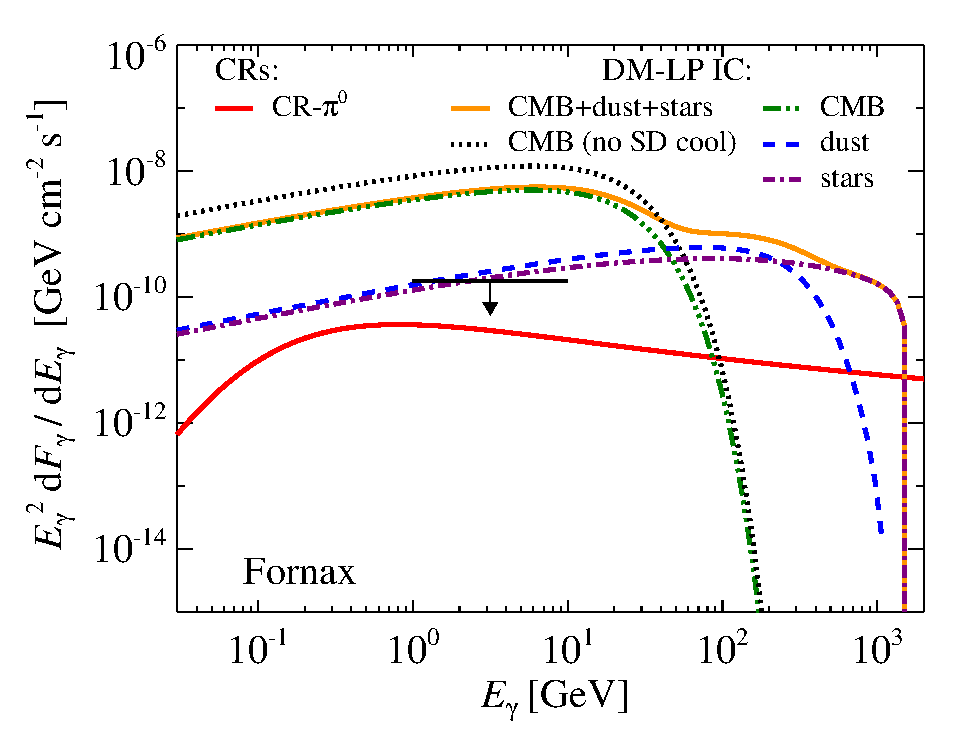
\includegraphics[width=0.49\columnwidth]{figures/flux.IRcomp.v9.0.1deg.1.6T.SubMass.elmu.SF300.noMW.woGal.eps}
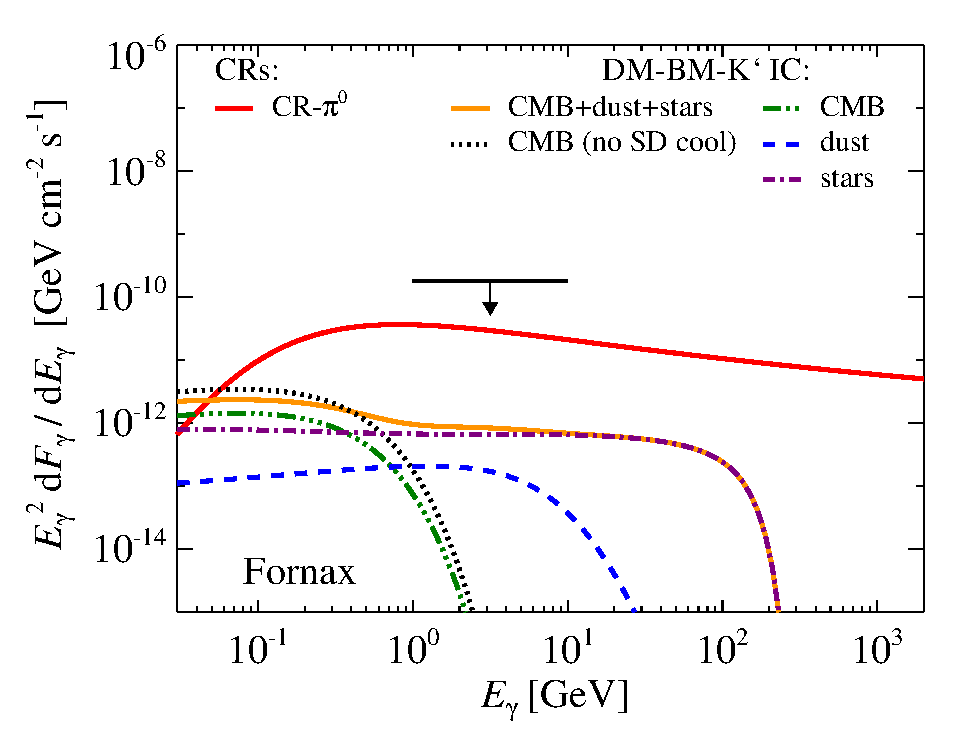
\includegraphics[width=0.49\columnwidth]{figures/flux.IRcomp.BMv9.0.1deg.SubMass.noMW.woGal.eps}
\caption{\it Comparing the flux from different inverse Compton
  upscattered radiation fields. We show the differential inverse
  Compton emission induced by leptophilic DM in the left panel and by
  the $\Kp$ benchmark model in the right panel. The contribution from
  each individual radiation field from top line to bottom line; CMB
  (green dashed-double-dotted), dust (blue dashed), stars (purple
  dashed-dotted). The sum of the three components are shown with the
  orange solid line. The black dotted line represents the upscattered
  CMB photons without any cooling from stars and dust. The red solid
  line show the CRp induced gamma-ray flux. The black arrow show the
  differential upper limit from Fermi \cite{2010ApJ...717L..71A}. All
  fluxes are calculated for the Fornax cluster within $\rvir$ using a
  point spread function of $0.1\deg$. The boost from Sommerfeld and
  substructures is about 130 and 570, respectively.}
 \label{fig:IR_comp}
\end{minipage}
\end{figure*}

It is also interesting to compare the total contribution from the LP
model, the brightest BM model ($\Kp$), and the CRp induced emission. In
Fig.~\ref{fig:flux_int} we show the integrated flux from Fornax for
our different gamma-ray models and compare it to the unresolved
integrated flux upper limit on Fornax set by Fermi-LAT where they
averaged the flux over the energy range $0.2-100\,\gev$ assuming a
spectral index of 2. Again we are overproducing the upper limits,
although only with a factor 10 which is about a order magnitude less
constraining than the differential flux in the energy range
$1-10$~GeV. From the figure one clearly see that the LP model is
dominating the entire gamma-ray energy range up to the DM mass of this
model of about 1~TeV. In addition it is interesting to note that the
flux the DM BM $\Kp$ model is above the predicted emission from the
CRps in the $1-100$~GeV energy regime accessible both to Fermi and
Cherenkov telescopes.

\begin{figure}
 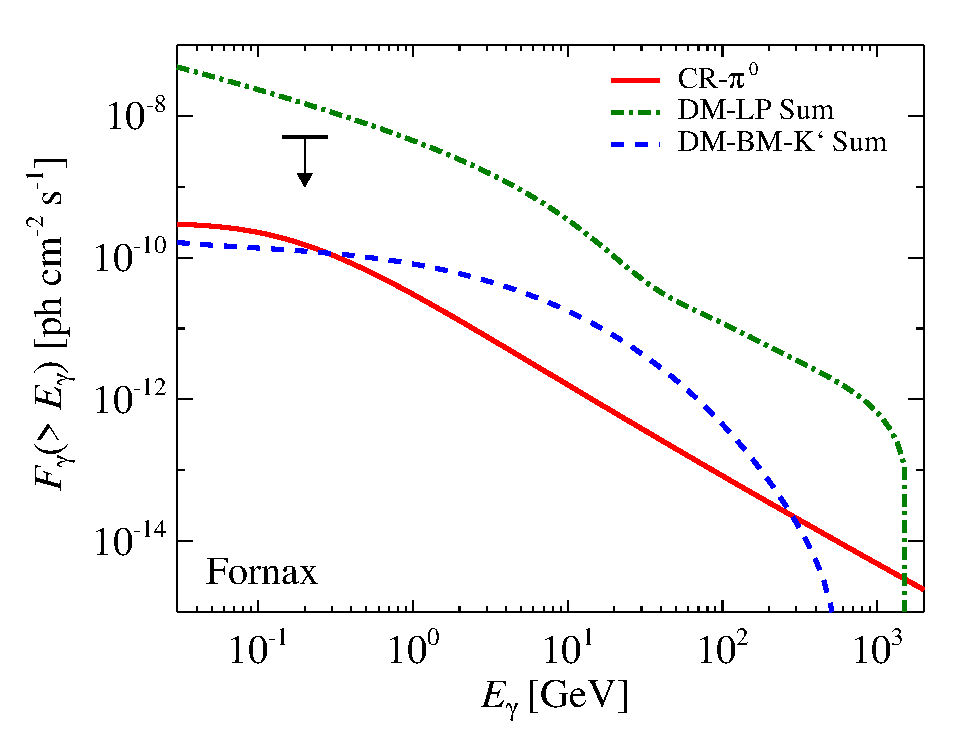
\includegraphics[width=0.99\columnwidth]{figures/flux.int.v9.0.1deg.1.6T.SubMass.SF300.IR2.noMW.woGal.eps}
\caption{\it Comparing the energy integrated flux from different
  models. We show the emission from; CRp induced emission (red solid),
  leptophilic models (LP) that include both final state radiation and
  IC upscattered CMB, dust and starlight (green dash-dotted), and
  benchmark $\Kp$ models (BM) include continuum emission, and IC
  upscattered CMB, dust and starlight (blue dashed). The black arrow
  show the integrated flux upper limit set by Fermi-LAT. The emission
  is calculated for the Fornax cluster using a point spread function
  of $0.1\deg$. The boost from Sommerfeld and substructures is about
  130 and 570, respectively. We find that LP models are dominating the
  total flux in the entire energy range, where the IC upscattered CMB
  photons overproduce the upper limit by a factor 3.}
 \label{fig:flux_int}
\end{figure}

We continue by comparing the estimated differential flux from Fornax
to three other clusters in Fig.~\ref{fig:clu_comp}; the close by well
studied Virgo cluster, the X-ray bright Perseus clusters, and the
massive merging Coma cluster. We find high DM induced gamma-ray fluxes
from both the Fornax and Virgo clusters, which highlight them as
promising targets for indirect DM searches. Note, however, that we
have used spatially unresolved upper limits, which is quite optimistic
for the angular extended Virgo cluster. It is quite striking how
constraining the upper limits for the Fornax cluster is compared to
the other clusters, especially in the $1-10$~GeV energy regime where
Fermi-LAT is most sensitive due to the maximized effective area. The
upper limits for Virgo and Perseus are background contaminated by AGN
activity from M87 and NGC 1267, respectively, and do not gain much
from the increased sensitivity. One should also note that the high CRp
induced flux from both Coma and Perseus is of the same magnitude as
the DM flux from LP models, making it difficult for indirect DM
searches in those clusters. Conversely is the Fornax cluster a great
target for indirect DM studies because the relative low gamma-ray flux
from CRps, absents of an active AGN, and high DM gamma-ray
flux. Actually, the Fermi-LAT 3 year data will be able to constrain
the smallest mass of substructures using the DM BM models. We have
also learned that the closest clusters are superior for DM searches
compared to further away clusters, even though the close by clusters
have a mass that is smaller. In fact, we can understand this by
looking at the luminosity-to-mass scaling relations. The gamma-ray
luminosity from the smooth density profile is given by
\begin{equation}
L_{\gamma,\rmn{sm}} \propto \int \dd V \rho(r)^2 \propto \frac{c^3}
{\left[\log\left(1+c\right)-c/(1+c)\right]} \propto \mvir^{0.83}\,,
\end{equation}
and the total DM luminosity including boost factors for the LP and
the BM models are given by
\begin{eqnarray}
\label{eq:LP_scaling}
L_{\gamma,\rmn{LP}} &=& L_{\gamma,\rmn{smLP}} \B_\rmn{LP} \propto \mvir^{0.73}\qquad
\,\,\,\,\,\,\rmn{and}\\
\label{eq:BM_scaling}
L_{\gamma,\rmn{BM}} &=& L_{\gamma,\rmn{smBM}} \B_\rmn{BM} \propto  \mvir^{1.06}\,,\qquad
\rmn{where} \\
B_\rmn{LP}&=&B_\sfe B_\sub \propto \mvir^{-1/3}\mvir^{0.23} \propto
 \mvir^{-0.1}\,,\\
B_\rmn{BM}&=&B_\sub \propto \mvir^{0.23}\,.
\end{eqnarray}
Hence increasing the mass with a factor two doubles the luminosity,
but increasing the distance by a factor two decrease the flux with a
factor four. It is also usefull to relate the luminosities to a more
model independent variable as the maximum circular velocity given by
\begin{eqnarray}
V_\rmn{max} &=& V_\rmn{circ}(r_\rmn{max})\qquad\,\,\,\,\,\,\,\,\,\rmn{where}\nonumber\\
V_\rmn{circ}(r)&=& \sqrt{\frac{G_\rmn{N}\,M(<r)}{r}}\qquad\rmn{and}\nonumber\\
\frac{\dd V_\rmn{circ}(r)}{\dd r} &=& 0\quad \Longrightarrow\quad r_\rmn{max}\,.
\end{eqnarray}
We find that $V_\rmn{max}=650\,\rmn{km/s}$ of a large $10^{15}\,\msun$
cluster, and $V_\rmn{max}=420\,\rmn{km/s}$ of a small
$4\times10^{13}\,\msun$ group.


\del{
\begin{eqnarray}
L_{\gamma,\rmn{sub tot}} \propto N\,L_{\gamma,\sub} \propto N\,M_\sub 
 \propto M_\sub^{\left(A+1\right)}\,\frac{\dd N_\sub}{\dd M} \propto  M^{A-0.9}
\end{eqnarray}
Assuming that the concentration $c$ decrease for increasing mass as it
does for the mass range $10^{12}-10^{14}\,\msun$ where
$L_{\gamma,\sub} \propto N\,M_\sub^A$, where $A<1$.
}

\begin{figure*}
\begin{minipage}{2.0\columnwidth}
 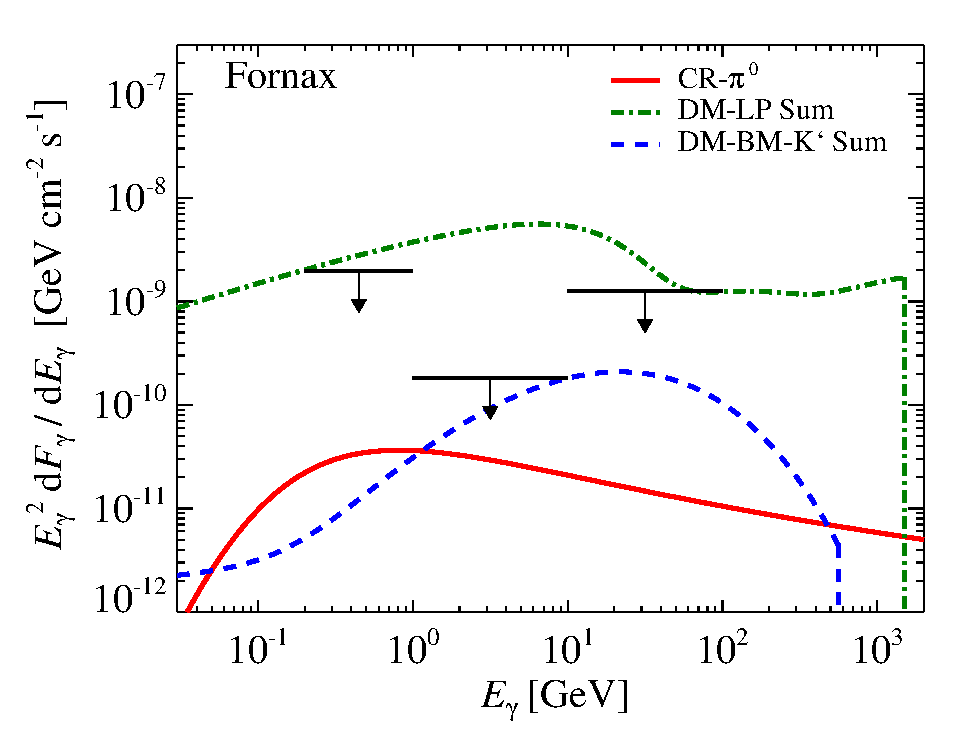
\includegraphics[width=0.49\columnwidth]{figures/flux.cluster.Fornax.v9.0.1deg.1.6T.SubMass.SF300.IR2.noMW.woGal.eps}
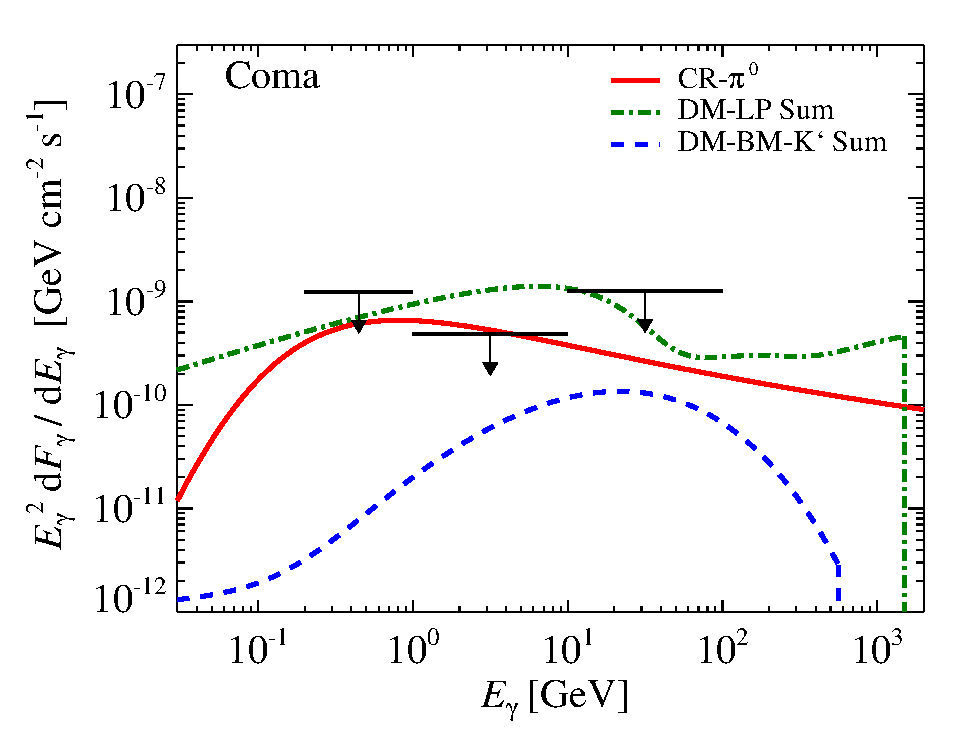
\includegraphics[width=0.49\columnwidth]{figures/flux.cluster.Coma.v9.0.1deg.1.6T.SubMass.SF300.IR2.noMW.woGal.eps}
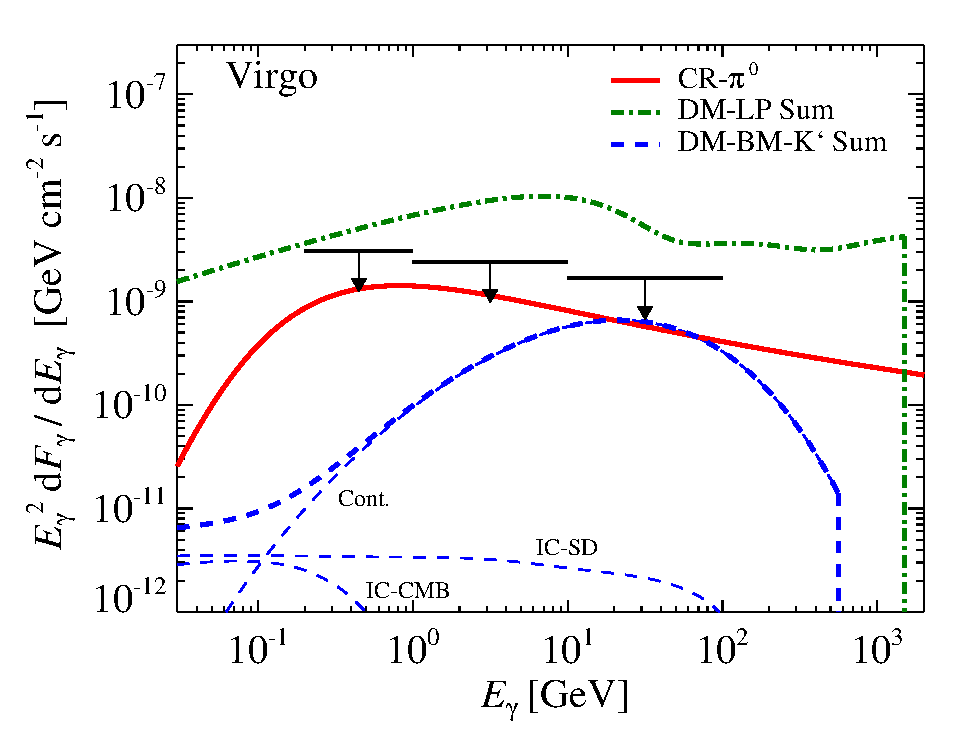
\includegraphics[width=0.49\columnwidth]{figures/flux.cluster.Virgo.v9.0.1deg.1.6T.SubMass.SF300.IR2.noMW.woGal.eps}
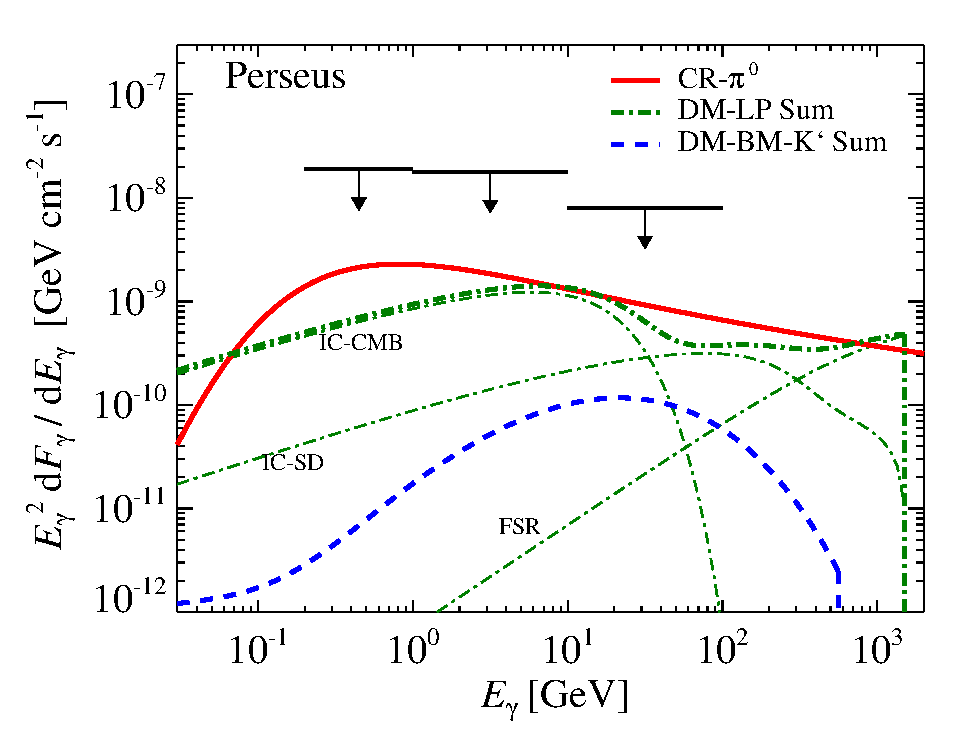
\includegraphics[width=0.49\columnwidth]{figures/flux.cluster.Perseus.v9.0.1deg.1.6T.SubMass.SF300.IR2.noMW.woGal.eps}
\caption{\it Comparing the emission from different clusters. We show
  the differential flux from four clusters; Fornax (upper left), Coma
  (upper right), Virgo (lower left), and Perseus (lower right). The
  different flux models; CRp induced emission (red solid), leptophilic
  models (LP) include both final state radiation and IC upscattered
  CMB, dust and starlight (green dash-dotted), and benchmark $\Kp$
  models (BM) include continuum emission, and IC upscattered CMB, dust
  and starlight (blue dashed). The arrows have colors matching each
  cluster and show the differential upper limits set by Fermi-LAT in
  the energy ranges $0.2-1$~GeV, $1-10$~GeV, and $10-100$~GeV from
  left to right. For visualization we offset the arrows by increasing
  the mean energy by 30\% in the opposite order as they appear in the
  figure, i.e. starting with Perseus. The flux from the clusters is
  integrated out to $\rvir$ using a point spread function of $0.1\deg$
  and includes the boost from substructures. We find that the lower
  GeV energy regime is most constraining, and induce upper limits on
  boost factors.}
 \label{fig:clu_comp}
\end{minipage}
\end{figure*}

As we have seen in this section the LP models overproduce both the
differential and integrated flux upper limits set by the Fermi-LAT for
several clusters. We can use these upper limits to enforce constraints
on the SFE and boost from substructures. As more sensitive experiments
and better upper limits emerge, we can start ruling out models that
give rise to boost factors that are manifested in the gamma-ray
flux. It is especially interesting is to constrain the SFE, where a
boost of 300 is required to explain the excess of electrons and
positrons observed in the vicinity of Earth by PAMELA/Fermi/HESS.  In
Fig.~\ref{fig:clu_comp} we use the estimated flux from four clusters
to constrain the SFE as well as the minimum mass of substructures
where $M_\rmn{lim}\propto\mvir^{0.226}$. As expected, the Fornax
cluster is the most constraining cluster by far, although the current
upper limits are not good enough to rule out the boost from
substructures or SFE. Assuming that the electron and positron excess
is due to SFE DM matter, then in order not to overproduce the
differential upper limits set by Fermi-LAT in the energy range
$1-10$~GeV \footnote{We average the LP DM flux in the energy range
  $1-10$~GeV before we compare it to the upper limits.}  we can
constrain the smallest mass of substructures to $M_\rmn{lim}\gtrsim
10\,\msun$. Instead assuming the standard mass of the smallest
substructures of $M_\rmn{lim}\gtrsim 10^{-6}\,\msun$, we can constrain
the boost from SFE to about 4 in Fornax, corresponding to a maximum
SFE in the MW of about 10.


\begin{figure}%[t]
 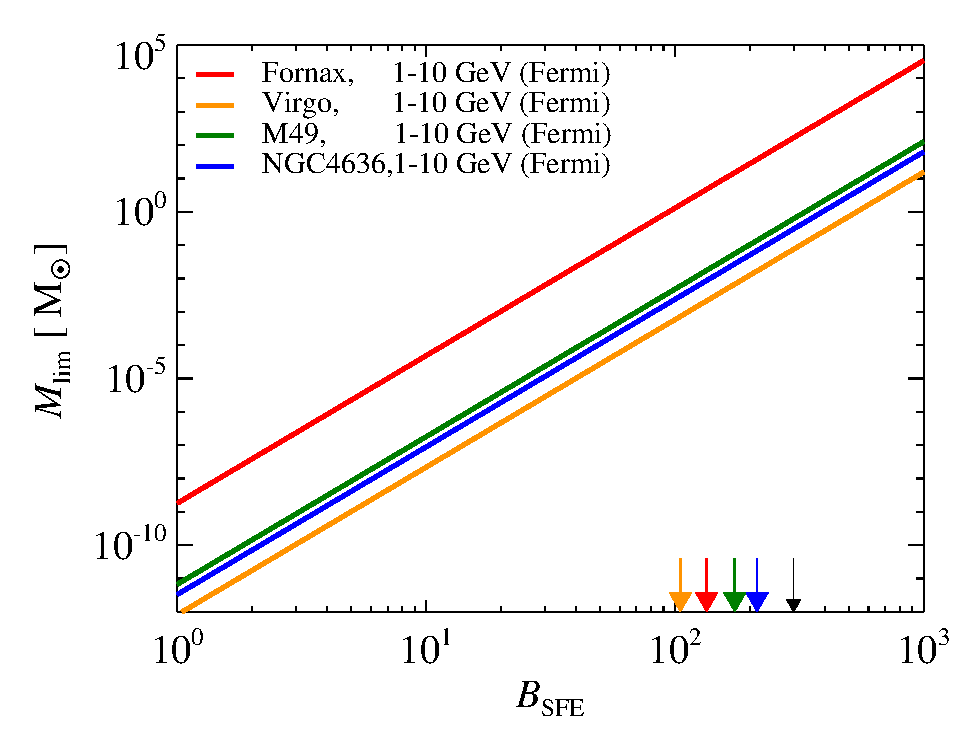
\includegraphics[width=0.99\columnwidth]{figures/LP.const.diff.v9.0.1deg.1.6T.SubMass.SF300.IR2.noMW.woGal.eps}
\caption{\it Constraining boost factors using flux upper limits. The
  leptophilic (LP) gamma-ray emission is derived within $\rvir$ using
  a point spread function of $0.1\deg$. In order not to overproduce
  the Fermi-LAT differential flux upper limits in the energy interval
  $1-10$~GeV the boost from substructures and Sommerfeld enhancement
  (SFE) is constrained for four clusters; Fornax (red), Virgo
  (orange), M49 (green), and NGC4636 (Blue). The SFE has been rescaled
  from 300 (refer to equation) that is required to explain the
  electron and positron excess observed at Earth with LP DM (black
  arrow). If the DM interpretation is correct, we can constrain the
  smallest size of halos to be larger than $10\,\msun$. However, if
  the smallest size of DM halos is $10^{-6}\,\msun$, we can constrain
  the SFE to about 4 in Fornax, corresponding to a maximum SFE in the
  MW of about 10.}
 \label{fig:boost_const}
\end{figure}


\section{Surface brightness profiles}
\label{sect:spatial}
The large angular extent of clusters on the sky in combination with
the small PSF of most gamma-ray probes ($\sim 0.1$~deg) suggest that
we would be able to probe the different spatial regimes of a
cluster. Especially important is the spatial distribution of the
gamma-ray emission as it bias upper limits derived for spatially
extended clusters where a simple density profile is often assumed. In
fact when DM substructures are included the total brightness profile
is almost flat and very different from the smooth halo distribution
with a steep outer brightness slope of $-5$.

In this section we investigate the gamma-ray surface brightness
profiles induced by both CRps and different models of DM in more
detail. We start by comparing the substructure included brightness
from different clusters in Fig.~\ref{fig:SB_clu}. As expected, we find
that the DM flux in all clusters follow the same smooth universal
shape imposed by the substructures. Even as far in as 1\% of $\rvir$
we are dominated by the substructures, which is due to the projection
of the outer cluster halo (see Sect.~\ref{sect:subst} for a longer
discussion). This implies that the spatial distribution of
annihilating DM induced emission is independent of the type of DM
model, and can not be used to separate different models. The
normalization for the BM model is determined by $\bsub
L_{\gamma,\rmn{BM}}^{1/3} \propto \mvir^{0.5}$, which explains the
factor three difference in normalization between the most massive
cluster Coma and the least massive cluster Fornax with a mass ratio of
about 10. The flux from the LP model show a smaller spread in the
normalization which is due to the additional contribution from SFE
with a negative mass trend, hence a normalization with a softer
mass-scaling of $\sim\mvir^{0.17}$. The surface brightness induced by
CRps mainly trace the gas profile of each cluster with an additional
enhancement in the center due to the expected large population of
CRps, hence we see a much larger spread in these profiles. It is
noticeable that Fornax show such a small surface brightness. However,
it is explained by the low gas density outside the BCG and the less
abundant CRp population in the relative small cluster compared to a
more massive cluster \cite{2010MNRAS.409..449P}. In fact, only the
very inner part of Fornax is dominated by a large gamma-ray flux from
CRps, which however, is neglible compared to the flux withing
$\rvir$. This is the reason why Fornax is such a good target for
indirect DM searches, and competitive to DM searches in dwarf
galaxies. Although, it might be a problem for Cherenkov telescopes
looking for a DM in the center of Fornax.

\begin{figure}
 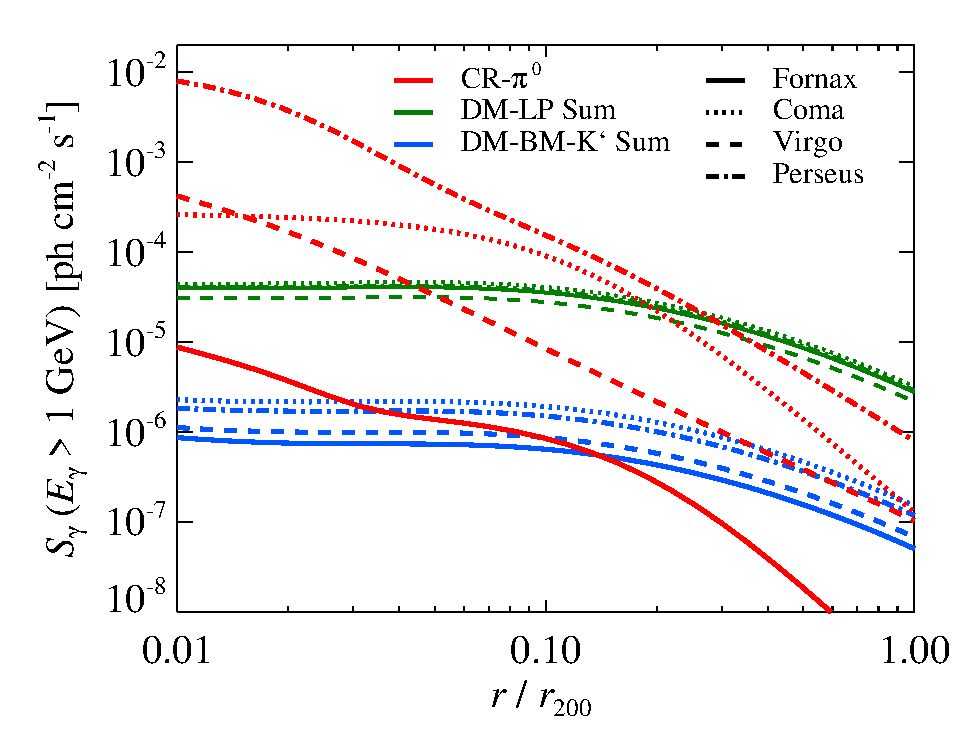
\includegraphics[width=0.99\columnwidth]{figures/SB.v9.1GeV.SF300.SubMass.elmu.eps}
\caption{\it Comparing the surface brightness from different
  clusters. We show the CRp induced emission (red), leptophilic
  emission (green), and emission from the $\Kp$ benchmark model
  (blue). The surface brightness above 1~GeV is derived using a very
  small point spread function ($\psf=10^{-5}\deg$). The
  different linestyles each represent a cluster; Fornax (solid), Coma
  (dotted), Virgo (dashed), and Perseus (dash-dotted). The boost from
  Sommerfeld and substructures is about 130 and 570,
  respectively. Notice the very similar shape and normalization of the DM
  models, while the CRps have a much larger scatter in the profiles.}
 \label{fig:SB_clu}
\end{figure}

To quantify the impact of substructures on the spatial profiles in
more detail we again turn to the Fornax clusters and show in
Fig.~\ref{fig:SB_sub} a comparison of surface brightness profiles with
and without substructures. It is quite remarkable how flat the
profiles including substructures are compared to the ones
without. This implies that the relative flux within the PSF in the
center is comparable to the outer parts, which should increase the
signal-to-noise significantly. If we assume that substructures for
some reason are suppressed in the Fornax cluster, then the expected
signal from DM is swamped by astrophysical backgrounds over the entire
extent of the cluster, even though Fornax has one of the highest
ratios of DM/CRp gamma-ray brightness.

\begin{figure}%[t]
 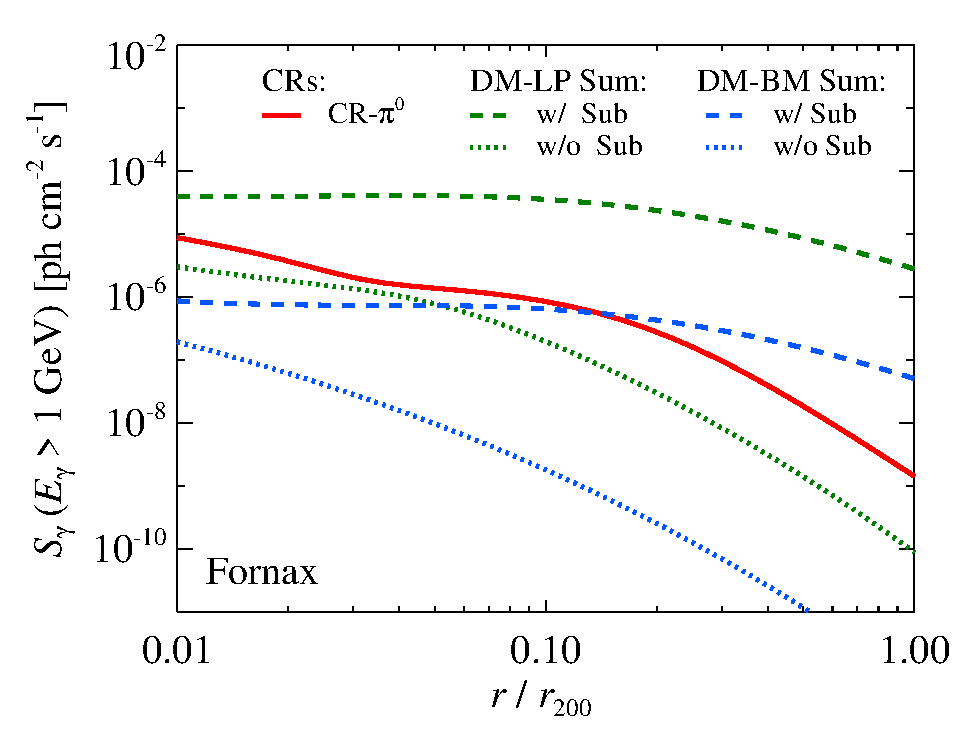
\includegraphics[width=0.99\columnwidth]{figures/SB.resolved.v9.1GeV.SF300.noSuB.vs.SubMass.elmu.eps}
\caption{\it The impact of substructures on surface brightness. We
  show the surface brightness at 1~GeV for the Fornax cluster using a
  very small point spread function of $10^{-5}\deg$ that reveals the
  details of the spatial profiles. The emission induced by CRps is
  denoted by the red solid line, the leptophilic models by green
  lines, and the DM $\Kp$ benchmark model by blue lines. The dashed
  line show the brightness where the boost from substructures is
  included while the substructures are excluded in the dotted
  line. The boost from Sommerfeld and substructures is about 130 and
  570, respectively. Notice the nearly flat profiles when
  substructures are included, and the relative large boost at a
  percent of $\rvir$.}
 \label{fig:SB_sub}
\end{figure}

NEED TO REWRITE, JUMPING BACK AND FORTH BETWEEN PANELS In order to
learn about the spatial distribution of the DM flux in various
clusters for different DM models and associated gamma-ray components,
we show in the left panel of Fig.~\ref{fig:SB_clu_nosub} the
brightness profiles for the smooth DM distribution for the same four
representative clusters that was shown previously in
Fig.~\ref{fig:SB_clu}. In addition, we show the spatial dependence of
the individual gamma-ray components for the Fornax cluster in the
right panel. We find that the spatial distribution of the DM emission
at 1~GeV in the outer parts of the all clusters have the same
shape. The shape trace the underlying density slope of $-3$, which is
expected for IC upscattered CMB photons. This picture is confirmed by
the components study in the right panel that show the neglible
contribution from the IC upscattered light from SD at this
energy. Since the surface brightness from BM models are dominated by
the continuum emission at each radial bin in all clusters, we see that
the total DM emission follows the projected density profile over the
entire clusters. The LP model, however, give rise to a much flatter
profile in the central parts of the clusters. This is due to the IC
upscattered CMB photons that are upscattered on an electron and
positron population that suffers from efficent cooling on light from
SD. The IC emission from SD photons have a rather steep spectrum in
the center that follows the projected density profile which is
explained by the SD dominated cooling that cancels the spatial
dependece from the SD spectrum. In the left panel we also find some
variation in the profiles for the different clusters in the central
parts. Especially in the Fornax cluster, where we find a factor two
larger flux compared to the other clusters. This is due to more
efficient SD cooling of the dominating IC upscattered CMB photons in
Fornax; a low X-ray luminous cluster has a low energy density in
starlight and dust in our semi-analytic SD model. However, note that
the surface brightness from the SD component is suppresses at the
relative low energy of 1~GeV.  Since there is no enhancement from the
substructures, the overall mass normalization of the LP DM model has a
marginally negative trend $\sim\mvir^{-0.06}$. Hence, we only see a
very small difference in outer parts of the different clusters from
these type of models. The BM DM models have a normalization of
$\sim\mvir^{0.27}$, hence more massive clusters show a slightly higher
surface brightness. As also noticed in previous figure, the flux from
DM without substructures is dominated by the CRp induced emission for
all clusters.

\begin{figure*}
\begin{minipage}{2.0\columnwidth}
  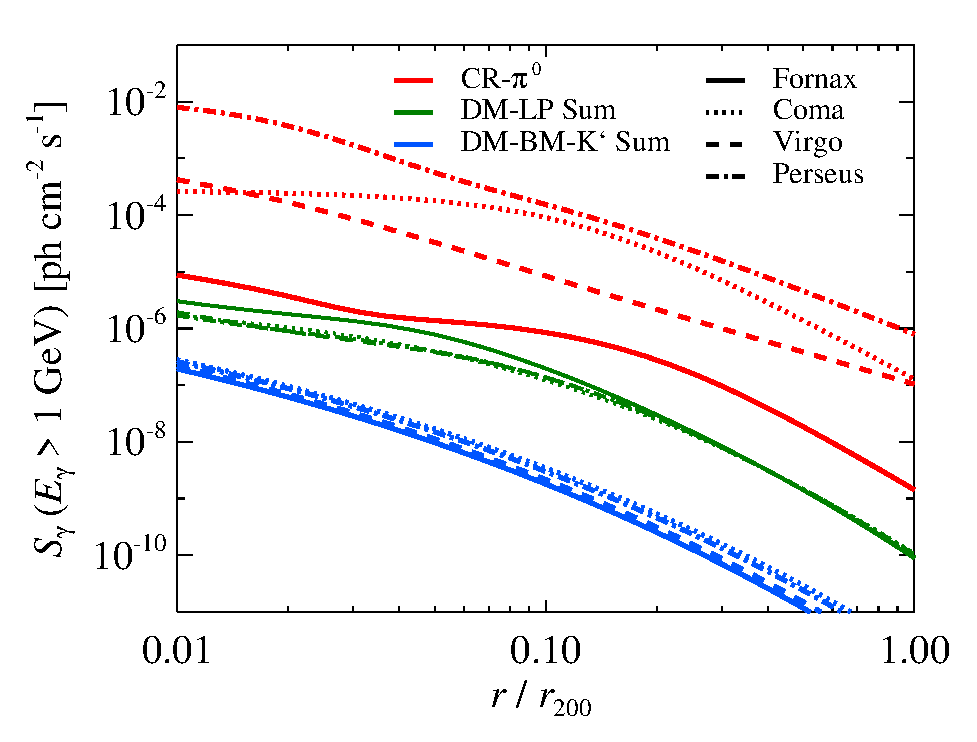
\includegraphics[width=0.49\columnwidth]{figures/SB.v9.1GeV.SF300.noSuB.elmu.eps}
  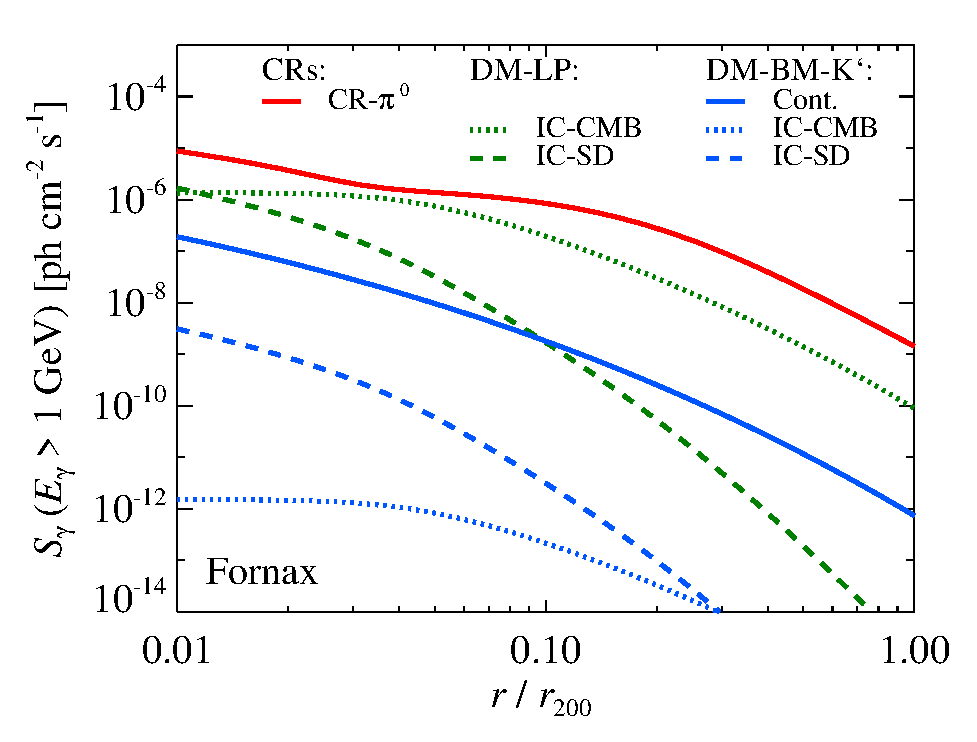
\includegraphics[width=0.49\columnwidth]{figures/SB.fornax.v9.1GeV.SF300.noSuB.elmu.eps}
\caption{\it The surface brightness without substructures. We show the
  CRp induced emission (red), leptophilic emission (green), and
  emission from the $\Kp$ benchmark model (blue). The surface
  brightness above 1~GeV is derived using a very small point spread
  function ($\psf=10^{-5}\deg$). LEFT PANEL: compare the
  surface brightness for different clusters; Fornax (solid), Coma
  (dotted), Virgo (dashed), and Perseus (dash-dotted). RIGHT PANEL:
  compare different emission components in Fornax; dotted lines show
  the inverse Compton (IC) upscattered CMB photons, dashed lines show
  the IC upscattered photons from stars and dust, and blue solid line
  show the continuum emission from the $\Kp$ benchmark
  model.}
 \label{fig:SB_clu_nosub}
\end{minipage}
\end{figure*}

In Sect.~\ref{sect:spatial} we saw that the spectral distribution of
the gamma-ray flux from the LP model were dominated at high energies
of $100\,$~GeV by final state radiation and the IC upscattered
starlight and dust, while the BM models were mainly dominated by the
continuum emission. These high energies are reachable by both
Fermi-LAT and Cherenkov telescopes, thus important observationally. We
therefore show in Fig.~\ref{fig:SB_IACTs} the surface brightness above
$100\,$~GeV for a realistic PSF of $0.1\deg$ where we include the
boost from substructures. We look at two clusters with an expected
high DM signal; the relative small Fornax cluster and the massive
close by Virgo cluster Both clusters show a very flat brightness
profile within about 10\% of $\rvir$, due to both the effect from
substructures and the smoothening over the PSF. The CRp induced
emission also show a smoothing in the central parts due to the PSF. In
the outer part of the Fornax cluster the CRp flux is suppressed
compared to the substructure boosted DM flux, where the LP model is
over three orders of magnitude larger. Although, it should be noted
that there are large uncertainties in the gas density profile used to
estimate the CRp surface brightness (see Fig.~\ref{fig:dens_fornax}
for more details).

\begin{figure*}
\begin{minipage}{2.0\columnwidth}
  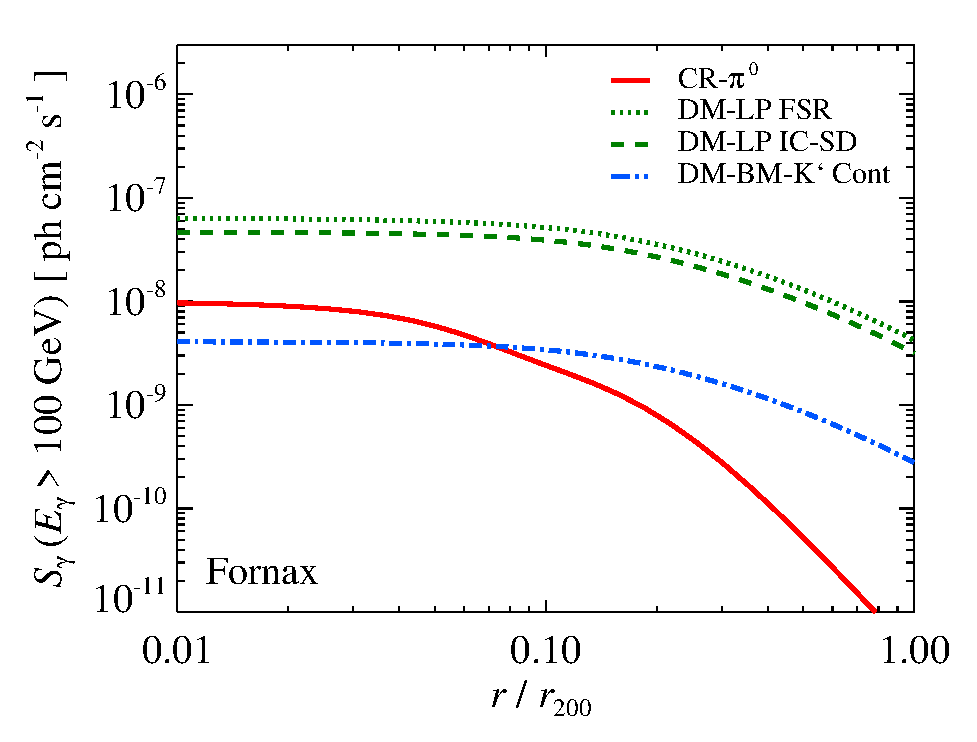
\includegraphics[width=0.49\columnwidth]{figures/SB.Fornax.v9.SF300.SubMass.elmu.eps}
  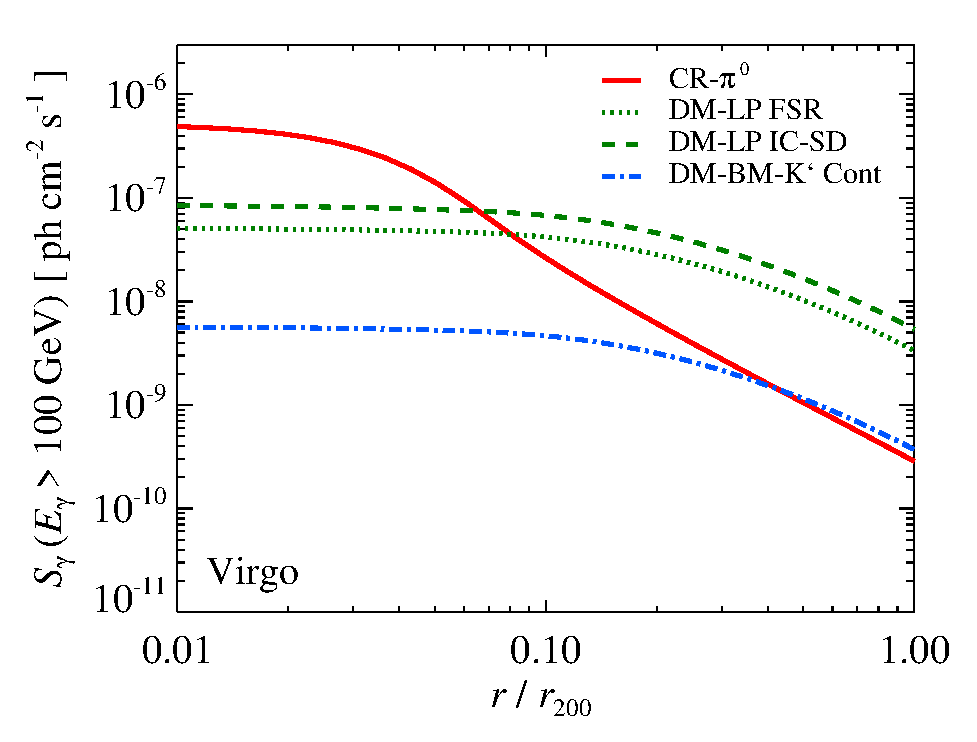
\includegraphics[width=0.49\columnwidth]{figures/SB.Virgo.v9.SF300.SubMass.elmu.eps}
\caption{\it Surface brightness predicted for Cherenkov telescopes at
  high energies. We show the emission above $100$~GeV and include the
  boost from substructures. We use a point spread function of
  $\psf=0.1\deg$ that is typical for both Cherenkov
  telescopes as well as the Fermi-LAT at this energy. Left panel show
  the Fornax cluster and right panel the Virgo cluster. The gamma-ray
  emission is derived for the following components; CRps (red solid),
  continuum emission from the DM $\Kp$ benchmark model (blue
  dash-dotted), as well as final state radiation (green dashed) and
  inverse Compton upscattered dust and starlight (green dotted) from
  leptophilic DM.}
 \label{fig:SB_IACTs}
\end{minipage}
\end{figure*}



\section{Predictions and observational limits}


In this section, we compute the expected $\gamma$-ray fluxes from DM
annihilation and CR interactions of the brightest clusters of the X-ray flux
complete sample in the local universe. We confront these predictions to upper
limits obtained by Fermi 1.5-year data and conclude on the viability of the
underlying models and perspectives for the next years of Fermi observations.

\begin{figure*}
  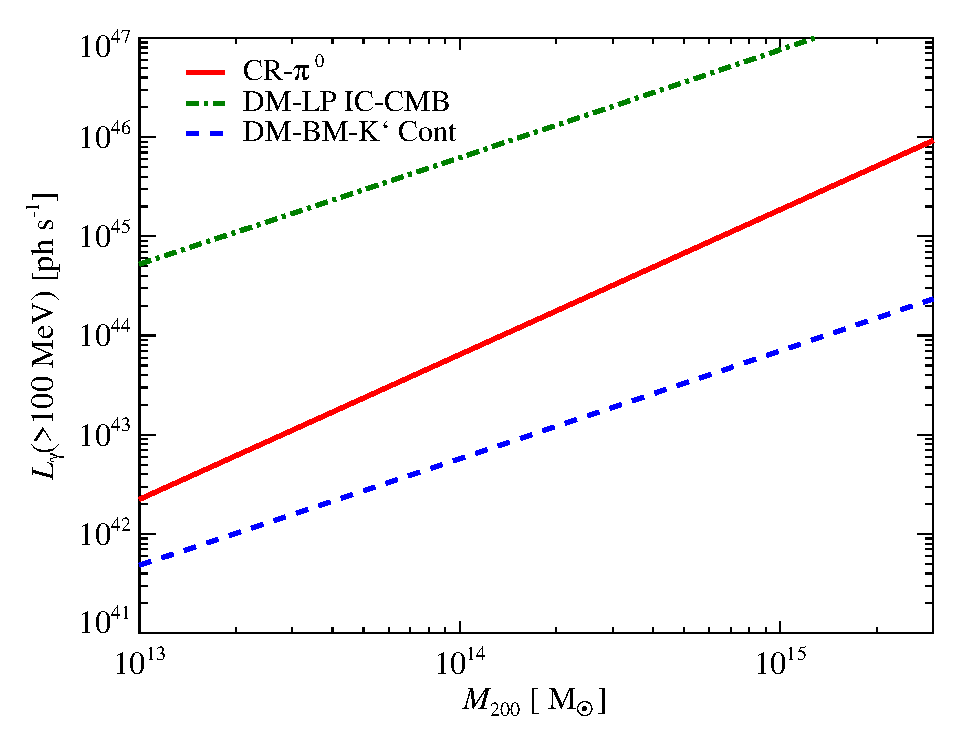
\includegraphics[width=0.99\columnwidth]{figures/MLscaling.100M.eps}
  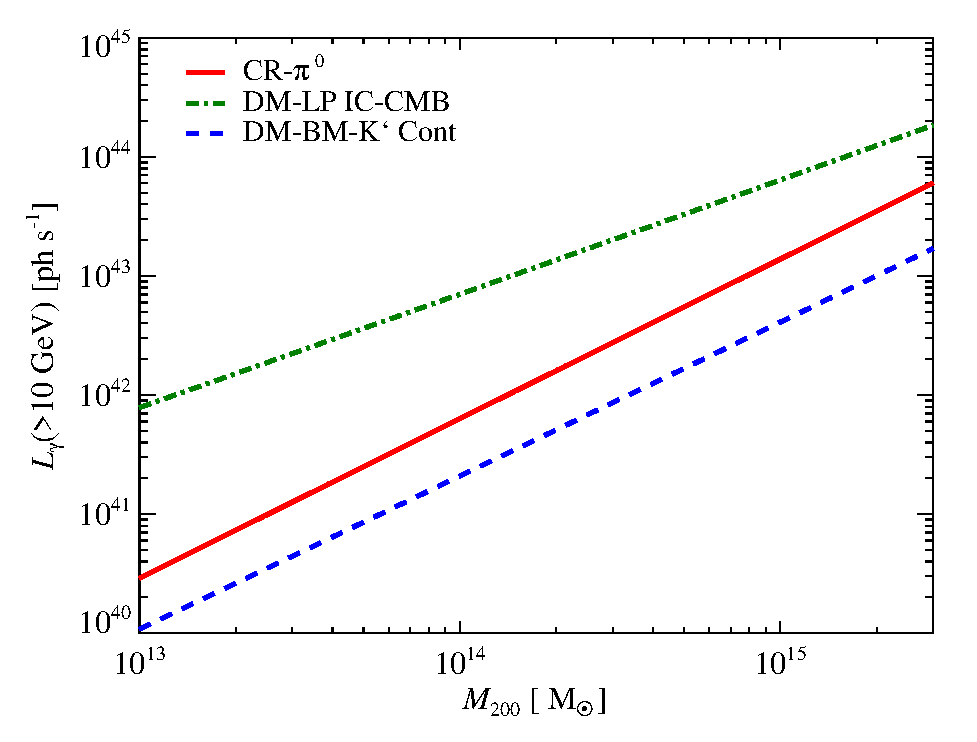
\includegraphics[width=0.99\columnwidth]{figures/MLscaling.10G.eps}
  \caption{\it Scaling relations of the cluster's virial mass $M_{200}$ and the
    $\gamma$-ray luminosity for energies $E_\gamma>100$~MeV (left) and
    $E_\gamma>10$~GeV (right).  Shown are the relations for the CR-induced
    emission that is dominated by pion decay resulting from hadronic CR
    interactions (solid), the leptophilic model of DM annihilations that
    includes the scaling of the substructure and Sommerfeld boost factors with
    custer mass from Equation~(\ref{eq:LP_scaling}) (dash-dotted) as well as the
    benchmark model $K'$ of DM annihilation that includes the scaling of the
    substructure boost with cluster mass of Equation~(\ref{eq:BM_scaling})
    (dashed). Note that the scaling of this particular benchmark model is
    indicative for all (non-Sommerfeld enhanced) DM annihilation models while
    the normalization depends on the particular cross-section and neyralino
    masses.}
\label{fig:lum_mass_scaling}
\end{figure*}

First we focus on $\gamma$-ray flux-cluster mass scaling relations for DM
annihilation and CR induced emission in Fig.~\ref{fig:lum_mass_scaling}.  The
mass scaling of the substructure boost steepens the intrinsically shallower DM
annihilation relation of benchmark models (Equation~(\ref{eq:BM_scaling})) while
this steepening is in fact over-compensated by the inverse mass scaling of the
Sommerfeld boost in leptophilic models that prefers smaller halos with a larger
ratio of $c/v_\mathrm{circ}$ (Equation~(\ref{eq:LP_scaling})). In contrast, the
CR scaling relation is considerably steeper as shown by reference
\cite{2010MNRAS.409..449P}. [ANDERS: add CR scaling formula] This implies
already a general strategy to minimize the CR-induced foreground for DM
annihilation and argues for very nearby groups. We note that these simulations
do not include AGn feedback that is thought to furthermore reduce the baryon
fraction in groups relative to that in clusters \cite{2008ApJ...687L..53P}. The
resulting smaller target density for hadronic CR interactions will furthermore
steepen the $L_\gamma-M$ relation of CR induced emission, making the case for
groups even stronger.

\begin{figure*}
\begin{minipage}{2.0\columnwidth}
  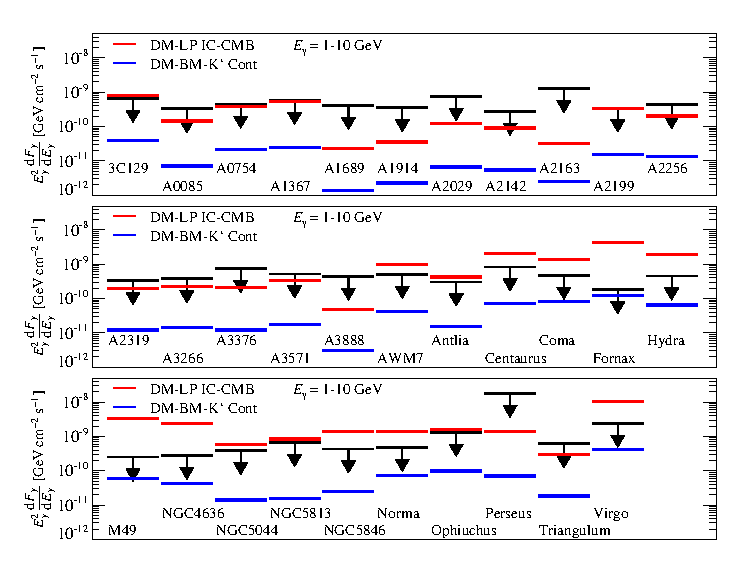
\includegraphics[width=0.99\columnwidth]{figures/Fermi.comp.DM.eps}
  \caption{\it Fermi flux upper limits are contrasted to the predicted DM
    gamma-ray flux. We show the mean differential flux in the energy range
    $E_\gamma=1-10$~GeV for 32 clusters. The Fermi-LAT upper limits are shown
    with black arrows. The predicted fluxes are derived from the dominant
    inverse Compton-scattering of CMB photons in a leptophilic DM model (red),
    and the continuum emission from the DM $\Kp$ benchmark model
    (blue). Assuming a boost factor due to substructures that has a mass
    spectrum extending down to Earth masses, the expected leptophilic fluxes are
    ruled out by lower upper limits in 14 of the clusters, with the strongest
    constraints set by Fornax and M49. We can not yet constrain the benchmark
    models, although our predictions are approaching the upper limits and will
    allow to test these in the upcoming years with better data.}
 \label{fig14}
\end{minipage}
\end{figure*}

Figure~\ref{fig14} compares Fermi upper limits on the $\gamma$-ray flux with
predictions of DM annihilation fluxes in the leptophilic and benchmark models.
To obtain the $\gamma$-ray fluxes, we scale the virial mass of clusters in the
extended HIFLUGCS catalogue \cite{2002ApJ...567..716R} with our scaling
relations of Equations~(\ref{eq:BM_scaling}) and (\ref{eq:LP_scaling}).  We
assume a boost factor due to substructures that has a constant contribution per
decade in substructure mass and has a mass spectrum extending down to Earth
masses. Fermi limits rule out the leptophilic models in their present form with
the mentioned assumptions in 14 clusters, and limit the boost from Sommerfeld
enhancement to less than 4 [?] in Fornax. Assuming universality, this limits the
Sommerfeld boost in the MW to less than 10 (see Fig.~\ref{fig:boost_const}).
The flux level of the Fermi limits are an indirect measure of the ambient
background flux in the $\gamma$-ray sky and/or the presence of strong point
sources such as AGN in the immediate vicinity of the cluster position. Hence, the ratio of
the Fermi upper limits to the predicted annihilation fluxes,
$F_{\mathrm{UL}}/F_{\mathrm{scal}}$, is a good indication of the best cluster
candidates for indirect DM experiments. We identify Fornax, M49, NGC4636, and
Virgo to be prime candidates. Note however, that Virgo extends of $7\deg$ over
the sky which implies a lower surface brightness and lower signal-to-noise.
Fermi limits on individual clusters are expected to improve as $\sqrt{T/1.5
  \mathrm{yr}}$, where $T$ is the total elapsed time of the Fermi mission. We
emphasize that the very inhomogeneous distribution of $F_{\mathrm{UL}}/
F_{\mathrm{scal}}$ makes it unlikely to dramatically improve the limits through
a stacking analysis as the weak signal will dilute the average constraints.
Assuming the projected sensitivity of the future Cherenkov telescope array (CTA)
of [ANDERS: value?], we note that it will be difficult to detect the DM
annihilation signal from clusters without a Sommerfeld boost by Cherenkov
telescopes. This is because the boost from substructures is extended while the
sensitivity of Cherenkov telescopes drops linearly with radius outside the point
spread function.

\begin{figure*}
\begin{minipage}{2.0\columnwidth}
  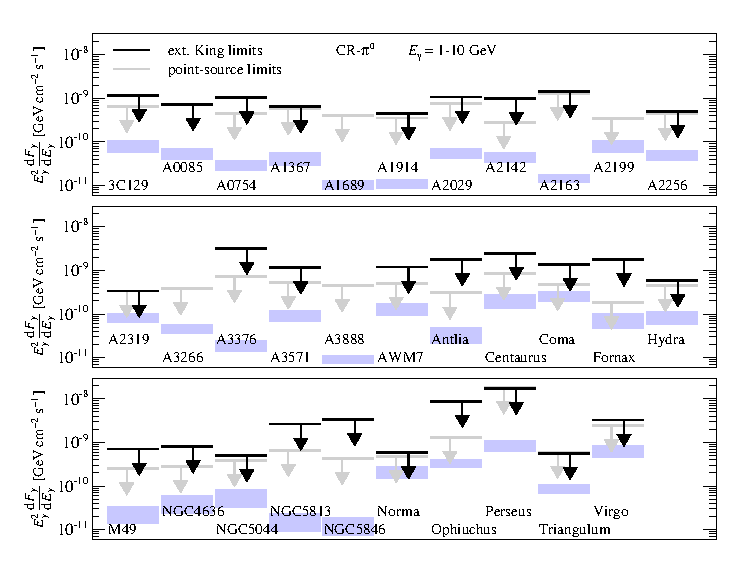
\includegraphics[width=0.99\columnwidth]{figures/Fermi.comp.CR.diff.eps}
  \caption{\it Fermi-LAT flux upper limits are contrasted to the predictions by
    the semi-analytic Pinzke and Pfrommer model for CRp induced gamma-ray
    emission. We show the mean differential flux in the energy range
    $E_\gamma=1-10$~GeV for 32 clusters. The Fermi upper limits are shown with
    black arrows. The blue boxes show the gamma-ray emission from CRp-induced
    $\pi^0$-decay, where the upper bound shows the estimates for an optimistic
    model and the lower bound a more conservative model excluding point sources
    (see \cite{2010MNRAS.409..449P} for details). Note that our models are in
    perfect agreement with the derived upper limits from Fermi. Interestingly,
    the limits of Virgo, Norma, and Coma are closing in on our predictions and
    will enforce constraints on the hadronic models in the coming years.}
 \label{fig15}
\end{minipage}
\end{figure*}

In Fig.~\ref{fig15}, we compare Fermi-LAT flux upper limits to the flux
predictions by the semi-analytical Pinzke and Pfrommer model
\cite{2010MNRAS.409..449P} for CRp induced $\gamma$-rays that uses the
X-ray-inferred density profiles of clusters as an input. For consistency, we use
beta-model fits to ROSAT data of X-ray bright clusters for our $\gamma$-ray flux
estimates \cite{2002ApJ...567..71}). Hence these predictions are superior to
those that use luminosity-mass scaling relation to infer the expected
$\gamma$-ray flux---a method used by reference \cite{2010ApJ...717L..71A} to
compare to Fermi limits.  In this semi-analytic model, we employ the fact that
CRs accelerated at structure formation shocks and transported over cosmic time
exhibit a universal spectral form and an almost universal spatial
distribution. Depending on whether or not we account for the bias of
``artificial galaxies'' in cosmological simulations, we derive an optimistic or
conservative limit of the expected $\gamma$-ray emission from decaying pions
(bracketing our ignorance of the contribution of cluster galaxies to the overall
$\gamma$-ray flux from a cluster). Note that both models assume the maximally
allowed acceleration efficiency for strong shocks that transfer 50\% of the
shock kinetic energy to CRs and most likely will have to be corrected down if
this number is not realized at structure formation shocks. Secondly, these
simulations neglect active CR transport such as streaming and diffusion relative
to the gas, i.e. we assume that advective transport is the dominant one and CRs
are tightly coupled to the gas via flux-frozen magnetic fields tangled on
sufficiently small scales. Evidence from the statistics of radio halos suggests
that this might not be the case for relaxed clusters, arguing that CR streaming
in those objects could be responsible for a decrease in the central CR number
density. This effect would also reduce the expected $\gamma$-ray flux by up to a
factor of five \cite{2011A&A...527A..99E}. We note that the tightest Fermi
limits are obtained in the 1-10 GeV regime due to the largest effective area of
LAT there. In this energy band, the Fermi limits come close to the flux
predictions of Virgo, Coma and Norma. Using integrated flux limits from Fermi,
we arrive at very similar results.  We emphasize that by using our semi-analytic
modeling, the slight discrepancy of the scaling relation-based prediction with
the Fermi limit on Norma \cite{2010ApJ...717L..71A} is resolved: Norma simply
seems to be less bright than an average cluster of the same mass as Norma. The
insenstitive limit on Perseus comes about since the central AGN in NGC1275 has
turned on over the last years, making it hard to determine a comparable
limit as obtained from teh other clusters.

\begin{figure*}%[t]
\begin{minipage}{2.0\columnwidth}
 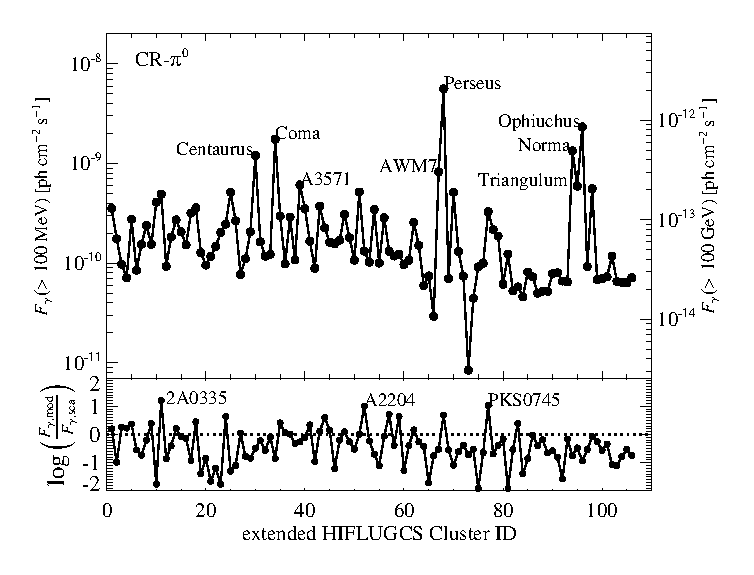
\includegraphics[width=0.99\columnwidth]{figures/Flux.comp.CR.eps}
 \caption{\it Comparison of the gamma-ray flux induced by CRps for the 106
   clusters included in the extended HIFLUGCS catalogue. The fluxes are
   calculated within $\rvir$, and are derived using a single beta profile for
   each cluster's gas density profile as obtained by ROSAT X-ray
   observations. The CR distribution follows the semi-analytically model derived
   by hydrodynamical cosmological cluster simulations \cite{2010MNRAS.409..449P}
   (see text for details). The upper panel shows the energy integrated flux
   above 100~MeV (left side) and above 100~GeV (right side), both as a function
   of HIFLUGCS cluster ID. The eight brightest clusters are labelled. The lower
   panel shows the relative difference between the gamma-ray flux predicted by
   the mass-luminosity scaling relation and to the flux computed using the
   semi-analytical model \cite{2010MNRAS.409..449P}. The name of the clusters
   with the largest offset are printed out, which correlate with cool core
   clusters.}
 \label{fig19}
\end{minipage}
\end{figure*}



if CC, then skewed towards large X-ray fluxes; X-ray emission good
proxies for gamma-ray emission --) The dust turns up at about a factor
100 lower than the stars --) The other figure show the spectral shape
of the IC-star with the same spectral shape as the dust, it shows the
same gamma-ray slope as the dust --) The reason why there is only a
factor 10 difference in the break in the gamma-ray emission between
the star and dust is related to the KN. In our CRp paper, the last
figure shows that at $\eg=100\,\tev$, the spectra is suppressed with
about a factor 10 (also depends on $\alpha_\e$). Since the dust
photons have a factor 10 higher energy, I expect this suppression at
about 10~TeV. For star photons the suppression should be at
100~GeV. So the star photons are definitely KN suppressed, which
explains the earlier break and the steeper slope.



%-) Consider having one figure where we compare the Einasto profile, to
%NFW, NFW w/ beta 0.6, and also the effect of a different concentration
%mass-scaling relation
%
%-) also, plot BM flux vs. psf, for models w/ and w/o substructures

\clearpage 

\section{Conclusions}

In this paper, we study the possibility for detecting $\gamma$-ray emission in
galaxy clusters. We consider benchmark and leptophilic models of supersymmetric
dark matter as well as cosmic ray induced pion decay which is thought to
dominate the astrophysical signal from clusters. Once supersymmetric cold dark
matter decouples from the expanding universe it streams freely and smooths over
any potentially present smaller scales. This imprints as a characteristic
minimum halo mass $M_\mathrm{min}$ into the hierarchy of structure formation and
should still survive until the present time as substructure within larger
halos. It turns out that the boost due to substructures dominates over the
smooth component for halo masses $M>10^3 \msun$ and contributes a constant
luminosity for each decade in halo mass. The ratio of halo-to-minimum subhalo
mass $M_{200}/M_\mathrm{min}$ is maximized for the largest systems that had time
to collapse and virialize since the Big Bang -- galaxy clusters. The
corresponding substructure boost can reach values exceeding $10^3$ which should
make nearby clusters the brightest DM annihilation sources after the Milky May
center and hypothetical very close-by DM substructures. Since the substructures
are distributed according to an Einasto profile, the contribution to the
annihilation emission from substructures peaks around the virial radius. This
implies an almost flat surface brightness profile of the annihilation emission
which makes it necessary to have the entire cluster in the field-of-view to take
advantage of the entire substructure boost.  This property makes it difficult to
detect DM annihilation emission without an enhancement of the particle physics
cross section over its standard value of $\sigma v\sim 3\times 10^{-26}
~\mathrm{cm}^3~\mathrm{s}^{-1}$ with imaging air Cherenkov telescopes due to the
spatially extended boost from substructures of angular extend $\sim
0.5-1\deg$. In contrast, the sensitivity of Cherenkov telescopes drops linearly
with radius outside the point spread function $\sim0.1\deg$.

We identify Fornax to be the best cluster/group candidate for indirect DM
studies as it is expected to emit the brightest annihilation flux and more
importantly, has a comparably low CR induced $\gamma$-ray flux.  This in
principle should allow to detect or constrain some benchmark models that have
been chosen for the large $\gamma$-ray flux yield with three-year Fermi data
(or constrain the substructure boost factor). Other nearby bright sources of the
extended HIFLUCGS sample of nearby bright X-ray cluster/groups are M49,
Centaurus, and NGC~4636.  The non-detection of $\gamma$-ray emission by Fermi in
a total of 14 clusters/groups (the mentioned clusters as well as Virgo, Coma,
Hydra, and Norma among others) considerably constrains leptophilic models for DM
annihilation which were introduced to explain the increasing positron-to-lepton
ratio beyond 10 GeV. Assuming that the minimum DM substructure mass extends down
to an Earth mass, we can rule out these leptophilic models based on the
non-observation of $\gamma$-rays in any of the fore-mentioned
clusters/groups. Alternatively, assuming the leptophilic models to be correct,
we limit the minimum substructure mass to $4~\msun$ in Fornax. Assuming
universality of the DM model, this corresponds to a minimum substructure mass of
$10~\msun$ in the Milky Way due to the larger Sommerfeld boost factor in smaller
mass halos which have a lower circular velocity which enhances the particle
cross section.

In this work, we thoroughly study the spectral emission characteristics of the
DM emission. In general there are different radiation mechanism that emit in the
$\gamma$-ray regime, namely (i) continuum emission following the hadronization
of the annihilating neutralinos in benchmark models which leads to the
production of charged and neutral mesons which decay finally into electrons,
neutrinos, and gammas, and (ii) inverse Compton (IC) emission by the leptons in
the final state which up-scatter radiation fields from the cosmic microwave
background, dust, and starlight, and (iii) final state radiation or internal
bremsstrahlung which dominates the highest energy emission close to the rest
mass of the self-annihilating neutralinos (if present in the model under
consideration). We construct a rather simple semi-analytic model for the spatial
and spectral distribution of dust and starlight in clusters which can be used
for the annihilation emission in galaxies with a different spatial profile.  We
find that in benchmark models, the continuum emission dominates over the IC
emission of any available radiation field. In the leptophilic models, where the
continuum emission is absent, the IC up-scattering of the CMB dominate below 30
GeV. For energies $30~\mathrm{GeV} \lesssim E_\gamma \lesssim 300~\mathrm{GeV}$,
the IC up-scattering of the dust emission dominates and is followed by the final
state radiation for energies up to $m_\chi c^2 \sim 1$~TeV. The IC emission of
starlight remains always subdominant. We stress, that the inclusion of the dust
and starlight radiation fields are important in the cooling function for the
leptons and a failure to do so biases the inferred CMB IC flux high by a factor
of two.

We substantially improve the modelling of the expected $\gamma$-ray signal from
pion-decay resulting from hadronic CR interactions with gas protons. We employ
the semi-analytic model of the CR spectrum and spatial distribution, recently
developed by \citet{2010MNRAS.409..449P} that is based on cosmological
hydrodynamical simulations that self-consistently follow the evolution of CRs in
cosmic structure formation. Adopting the model for all clusters in the HIFLUGCS
sample of flux-limited X-ray clusters, we compare the expected $\gamma$-ray
emission to that inferred from using $L_\gamma$-cluster mass scaling
relation. We note that the predictions of our ``optimistic'' model are perfectly
in agreement with Fermi upper limits for all clusters.  The hint of a tension
that the scaling relation modeling showed for Norma \citep{2010ApJ...717L..71A}
could not be confirmed due to the apparently lower gas density of this cluster
relative to the average.  As expected, the semi-analytic model adds ``scatter''
to the scaling relation and biases the $\gamma$-ray flux high for prominent cool
core clusters by up to a factor of 3.5 relative to the expectation from the
scaling relation. This is due to the high target gas densities and associated CR
densities in those cool cores that shape the spatial emission characteristic to
be very similar to that observed in thermal X-rays. We caution that these
predictions only apply for the case of negligible CR transport such as streaming
and diffusion relative to the gas and might be considerably modified in those
cluster that do not show an extended diffuse radio(-mini) halo that might point
to a centrally concentrated CR distribution \citep{2011A&A...527A..99E}. The CR
spectrum $E^2 dN/dE$ shows the characteristic pion bump at energies around
1~GeV. It is expected to dominate the DM annihilation signal in the benchmark
models for all clusters/groups but Fornax. We conclude that it will be possible
to rule out the leptophilic model with eight-years of Fermi data and start to
constrain some benchmark DM models. Hence this should nicely complement direct
and accelerator searches for the nature of dark matter.




\del{
Some of the results (should discuss what we want to emphasize):
O) the flux from annihilating DM is boosted by about a factor 1000 in
 clusters
O) flat surface brightness profiles with substructures
O) Fornax is a great target for indirect DM studies because the relative
 low flux from CRps and high flux from DM
O) the IC upscattered photons from stars and dust are dominated in the
 relevant energy regimes by the continuum emission for our DM
 benchmark models
O) Fermi 3 year data will constrain the smallest mass of substructures
 using the benchmark models
O) difficult to detect DM without a Sommerfeld boost with Cherenkov
 telescopes since the boost from substructures is extended while the
 sensitivity of Cherenkov telescopes drops linearly with radius
 outside the point spread function (CHECK)
O) we rule out the leptophilic models in present form in 14 clusters,
 and limit the boost from Sommerfeld enhancement in the MW to less
 than 10
--) the tightest limits on DM and CRps from Fermi are in the 1-10 GeV
 regime, where Fornax, M49, and NGC4636 are the most constraining
 "clusters" for the DM and Virgo, Coma and Norma are very close to the
 predictions for the CRps
O) we provide a rather simple model to calculate the spatial and spectral
 distribution of dust and stars in cluster (might be used for
 galaxies? with different spatial profile)
}

%------------------------------------------------------------------


\smallskip
Anders Pinzke acknowledges NSF grant AST 0908480 for support.


%-) Consider having one figure where we compare the Einasto profile, to
%NFW, NFW w/ beta 0.6, and also the effect of a different concentration
%mass-scaling relation
%
%-) also, plot BM flux vs. psf, for models w/ and w/o substructures


%%%%%%%%%%%%%%%%%%%%%%%%%%%%%%%%%%%%%%%%%%%%%%%%%%%%%%%%%%%%%%%
\vspace{-0.7cm}
\bibliography{bibtex/paper}
%\bibliography{apssamp}
%\bibliographystyle{apsrev4-1}

\clearpage
\appendix

{\it Spatial distribution -- stars and dust}\\ Our goal in this
section is to derive a simple spatial model for the distribution of SD
in galaxy clusters. For this reason we use stacked cluster
observations by Sloan in the $r$-band that trace the stars. We assume
that the dust trace the stars in the clusters, which should be
accurate to the order of magnitude estimate that we are interested in
here. The stacked surface brightness profiles in
\cite{2005MNRAS.358..949Z} are measured at redshift $z \sim 0.25$ with
an average mass of the clusters of $4.0\times10^{13}\,\msun$. The
profiles are build up out of three components; diffuse intracluster
light (ICL), galaxies, and the brightest cluster galaxy (BCG) in the
center of clusters. However, the total volume overlap of the ISM to
the cluster is very small compared to the ICL- and BCG overlap with
the cluster, thus the relative contribution of the galaxies to the IC
emission is suppressed. To remove this bias we cut out the galaxies
that have been smoothed over the cluster in the stacked analysis. In
Fig.~\ref{fig:SD_spatial} we show the SDSS stacked brightness profiles
as well as the fitted profiles\footnote{The measured brightness is
  converted into units of $\rmn{erg}\,\rmn{s}^{-1}$ using
  \cite{2010...book} $S(\rmn{mag}\,''^{-2}) =
  \mathcal{M}_\odot+21.572-2.5\rmn{log}_{10}S(L_\odot\,\rmn{pc}^{-2})$,
  where the sun's absolute magnitude in the $r$-band is given by
  $\mathcal{M}_\odot=27.1$ \cite{1998gaas.book.....B} and the
  luminosity of the sun by $L_\odot=3.85\,10^{33}
  \rmn{erg}\,\rmn{s}^{-1}$.}, both scaled with the unitless $\rvir$
normalized area to resembele the expected luminosity at radius
$r$. Our benchmark spatial model is shown with the solid black line,
and include the contribution from the ICL and BCG.



Instead of modelling the surface brightness with a de Vaucouleur
profile with the addition of a power-law, we use a double beta profile
model for simplicity of deprojection given by:
\begin{equation}
S_\sd (r_\bot)= \sum_{i=1}^2 \,S_i\, 
\left[1 + \left( \frac{r_\bot}{r_{\mathrm{c}_i}}\right)^2\right]
^{-3\beta_i + 1/2}\,,
\label{double_beta}
\end{equation}
where we found the following best fitted central brightness ($S_i$),
core radius ($r_{\mathrm{c}_i}$), and slope ($\beta_i$):
\begin{eqnarray}
 S_1&=&5.0\times10^{-6}\,\rmn{erg}\,\rmn{cm}^{-2}\,\rmn{s}^{-1},\,
r_{\mathrm{c}_1}=130\,\rmn{kpc},\,
\beta_1=0.54\nonumber\\
 S_2&=&3.9\times10^{-3}\,\rmn{erg}\,\rmn{cm}^{-2}\,\rmn{s}^{-1},\,
r_{\mathrm{c}_2}=2.8\,\rmn{kpc},\,
\beta_2=0.53\,.\nonumber\\
\label{fit_spatial_IR}
\end{eqnarray}
The 3D spatial profile is derived by deprojecting the surface
brightness in Eq.~(\ref{double_beta}) (see
e.g. \cite{2004A&A...413...17P} for details about the deprojection):
\begin{eqnarray}
  j(r)  = \sum_{i=1}^2 \frac{S_i}{2\pi\,r_{\mathrm{c}_i}}\,
  \frac{6 \beta_i - 1}{\left(1 + r^2/r^2_{\mathrm{c}_i}\right)^{3\beta_i}}\,
  \mathcal{B}\left(\frac{1}{2},3\beta_i\right)\,,
\end{eqnarray}
where $\mathcal{B}(a,b)$ denotes the beta-function
\cite{1965hmfw.book.....A}.

{\it Spectral distribution -- stars and dust} \\ Our goal in this
section is to derive a simple spectral model for SD in galaxy
clusters. Since the radiation from galaxies are expected to leak out
into the ICM, we expect similar spectral distributions, at least to
the order of magnitude that we are interested in here. Hence, we use
the IR to UV spectrum derived in \cite{2006ApJ...648L..29P} for a MW
type galaxy to characterize the spectral distribution of light from SD
in a cluster. Note, however, that we only keep the spectral shape, and
renormalize the spectral distribution using the luminosity from SD.

In Fig.~\ref{fig:SD_spectra} we show the spectral distribution of the
light from SD together with the CMB black-body distribution in a
galaxy cluster, both at the radius $r=0.071\rvir$ where the energy
density of the smooth light from SD (see Fig.~\ref{fig:SD_Edens})
equals the energy density of the CMB. We have renormalized both the
spectral data and the fitted spectra using the luminosity from stars
and dust individually (see the normalization section below for further
details).

We choose to fit the spectrum of the dust that peaks at about
$10^{-2}\,\ev$ with a double power-law, and the slightly wider
spectral distribution of the stars that peaks at about $1\,\ev$ with a
tipple power-law. We find the best fit spectra for the SD in a
cluster through:
\begin{eqnarray}
  \eph^2\frac{\dd^2 N_\ph}{\dd \eph \dd V}
  &\equiv& u_\sd(\eph) =  \sum_i N_i(\lx) u_i^\gal(\eph)\,,\nonumber \\ 
\rmn{where}\quad i&=&\{\rmn{stars,dust}\} \qquad \rmn{and}\\ 
% &=&  N_\dust(\lx) u_\dust^\gal(\eph) + N_\stars(\lx) u_\stars^\gal(\eph)  \nonumber \\ 
%  \\
  u_\stars^\gal(\eph) &=& \frac{23\,\rmn{eV}}{\rmn{cm}^3} 
  \left(\frac{1.23\,\rmn{eV}}{\eph}\right)^{1.9} \nonumber \\
  &\times&\left[1+\left(\frac{2.04\,\rmn{eV}}{\eph}\right)^{20}\right]
  ^{-\frac{1.9}{20}}\nonumber \\
  &\times& \left[1+\left(\frac{0.78\,\rmn{eV}}{\eph}\right)^{20}\right]^{-\frac{2.6}{20}}\,, \\
  u_\dust^\gal(\eph) &=& 
  \frac{40\,\rmn{eV}}{\rmn{cm}^3} 
  \left(\frac{0.0144\,\rmn{eV}}{\eph}\right)^{4.9}\nonumber \\
  &\times& \left[1+\left(\frac{0.0144\,\rmn{eV}}{\eph}\right)^{1.9}\right]^{-4.9}\,.
\end{eqnarray}


{\it Normalization}\\ The spatial and spectral distribution functions
of the light from SD in a cluster are both normalized with a constant
determined from the luminosity in each respective wavelength. The
specific energy density is given by
\begin{eqnarray} 
u_\sd(\eph, r) &=& \frac{j(r)}{j(0)}\,u_\sd(\eph) \nonumber\\
&=& \frac{j(r)}{j(0)}\,\sum_i N_i(\lx) u_i^\gal(\eph)\,,
\end{eqnarray}
where we fix the unitless normalization $N_i(\lx)$ using the total
energy of the light in SD  within $\rvir$:
\begin{eqnarray} 
  E_{i,\vir} &=& L_i \frac{\rvir}{c} \nonumber \\
  &=&N_i(\lx)\int_{\rvir} \int_i \,\frac{j(r)}{j(0)} 
  \frac{u_i^\gal(\eph)}{\eph}\,\dd V\dd \eph\,,\nonumber \\
 \rmn{for}\quad i&=&\{\rmn{stars,dust}\}\,.
\label{eq:E_SD}
\end{eqnarray}
Here we approximate the total energy of the photons within $\rvir$
($E_{i,\vir}$) with the luminosity $L_i$ \cite{2008A&A...490..547G}
times the typical timescale it takes for a photon to propagate through
the cluster (we assume that the cluster is optically thin). Once we
derived the SD luminosities for a well representative cluster, we use
a IR to X-ray scaling relation to estimate the luminosity from an
arbitrary cluster:
\begin{equation}
L_\ir=1.05\times10^{45}\,\rmn{erg\,s}^{-1}\,
\left(\frac{\lx}{10^{44}\rmn{erg\,s}^{-1}}\right)^{0.53}\,,
\label{eq:SD-X}
\end{equation}
where $\lx$ is the luminosity of the X-ray emitting gas within
$\rvir$.

The normalization constant for the starlight $N_\stars(\lx)$ is derived
in the following three steps: (1) We use the average apparent magnitude
in the $(r+i)$-band $m_{(r+i),0.25}\approx 15.5$
\cite{2005MNRAS.358..949Z} of a cluster with the average mass
$\mvir=4.0\times10^{13}\msun$ at a redshift $z=0.25$ to derive the
luminosity from the stars:
\begin{equation}
L_\stars=10^{\frac{m_\odot-m_{(r+i),0.25}}{2.5}}
\left(\frac{D_\clu}{D_\odot}\right)^2 L_\odot
\approx 7.1\times10^{44}\,\rmn{erg}\,\rmn{s}^{-1}\,,
\label{eq:L_star}
\end{equation}
where the apparent magnitude of the sun $m_\odot\approx -27.1$, the
distance to the sun $D_\odot=4.85\times10^{-6}\,\rmn{pc}$, the
luminosity of the sun $L_\odot=3.85\times10^{33}\,\rmn{erg\,s}^{-1}$,
and the distance to the cluster $D_\clu=1.26\times10^9\,\rmn{pc}$. (2)
We use the IR to X-ray scaling relation in Eq.~(\ref{eq:SD-X}) to derive
a more general form of the luminosity from stars in
Eq.~(\ref{eq:L_star}) that is valid for an arbitrary cluster mass. The
cluster X-ray luminosities are found in the extended HIFLUGCS
catalogue \cite{2002ApJ...567..716R} to which we have added the Virgo
cluster. (3) The normalization constant for the stars is
determined from the above steps together with Eq.~(\ref{eq:E_SD})
where we integrate over the cluster volume and spectral distribution
of the stars. It is given by
\begin{equation}
 N_\stars(\lx) = 1.2\times10^{-9}\,
\left(\frac{\lx}{10^{44}\rmn{erg\,s}^{-1}}\right)^{0.53}\,.
\label{eq:N_stars}
\end{equation}
Note that since the luminosities include the contribution from
galaxies, we have integrated the spatial distribution including
galaxies to derive the normalization. Once the normalization is fixed,
the SD energy densities are derived from the spatial distribution
where galaxies have been excluded.

The normalization constant for the dust $N_\dust(\lx)$ is derived in the
following four steps: (1) We use a cluster with the the average mass
$\mvir=4.0\times10^{13}\msun$ and estimate the X-ray luminosity from
the X-ray to mass scaling relations derived for the Representative
XMM-Newton Cluster Structure Survey (REXCESS) in
\cite{2009A&A...498..361P}:
\begin{equation}
\lx=1.18\times 10^{44}\,\rmn{erg\,s}^{-1}
\left(\frac{M_{200}}{10^{14}\msun}\right)^{1.81}\,,
\end{equation}
where we have used that $M_\rmn{200} \approx 1.58\,M_\rmn{500}$ for a
small cluster \footnote{We derive the factor 1.58 using
  $M_\rmn{200}/M_\rmn{500}$ for the clusters in the HIFLUGCS catalogue
  with a mass similar to $\mvir=4.0\times10^{13}\msun$ that we use to
  derive the luminosity from dust.}. (2) From the IR to X-ray scaling
relation in Eq.~(\ref{eq:SD-X}) we can now estimate calculate the
luminosity from the dust for a $\mvir=4.0\times10^{13}\msun$ cluster;
$L_\dust=4.7\times10^{44}\,\rmn{erg\,s}^{-1}$. (3) We generalize
Eq.~(\ref{eq:L_star}) to an arbitrary cluster mass using
Eq.~(\ref{eq:SD-X}) together with the cluster X-ray luminosities in
the extended HIFLUGCS catalogue. (4) The normalization constant for
the dust can now be determined from from the above steps together with
Eq.~(\ref{eq:E_SD}) where we integrate over the cluster volume and
spectral distribution of the dust. It is given by
\begin{equation}
 N_\dust(\lx) = 1.4\times10^{-9}\,
\left(\frac{\lx}{10^{44}\rmn{erg\,s}^{-1}}\right)^{0.53}\,.
\label{eq:N_dust}
\end{equation}
Note that since the luminosities include the contribution from
galaxies, we have integrated the spatial distribution including
galaxies to derive the normalization. Once the normalization is fixed,
the SD energy densities are derived from the spatial distribution
where galaxies have been excluded.

{\it Energy density}\\ The spatial distribution of the SD energy
density is an important quantity since it impacts the steady state
electron and positron spectra through cooling. A higher density of SD
in a cluster suppresses the spectra of the upscattering particles. With
the formalism presented above, we can now derive the energy density
from starlight and dust in a galaxy cluster through
\begin{eqnarray}
\label{eq:U_SD}
u_\sd(r) &=& \int \dd \eph \frac{\dd^2 N_\ph}{\dd \eph \dd V}\,\eph
=\int \dd \eph \frac{u_\sd(\eph, r)}{\eph}
\nonumber \\
&=&  \frac{j(r)}{j(0)}  \int \dd \eph \sum_i 
N_i(\lx) \frac{u_i^\gal(\eph)}{\eph}\,. \nonumber \\
\end{eqnarray}
In Fig.~\ref{fig:SD_Edens} we compare the energy densities from
different radiation fields in a galaxy cluster with the mass
$\mvir=4.0\times10^{13}\msun$. We use two different profiles for the
SD energy density, where the total profile includes the contribution
from the ICL, the BCG and all the galaxies, while the galaxies are
excluded in the smooth profile. We find that even for a cluster with a
relative small mass the energy density of the SD components dominates
over the CMB and the magnetic fields (with a central B field of 3~$\mu
G$) within about 10\% of $\rvir$. Outside this radius the CMB is
dominating the energy density of the cluster, hence the magnetic
fields are always subdominant in the cluster and can safely be removed
from cluster IC calculations for a reasonable central B-field and
spectral index. Note that in this work we keep the contribution
from B-fields to the total energy density for consistency.


%***********************************************



\begin{figure*}
\begin{minipage}{2.0\columnwidth}
 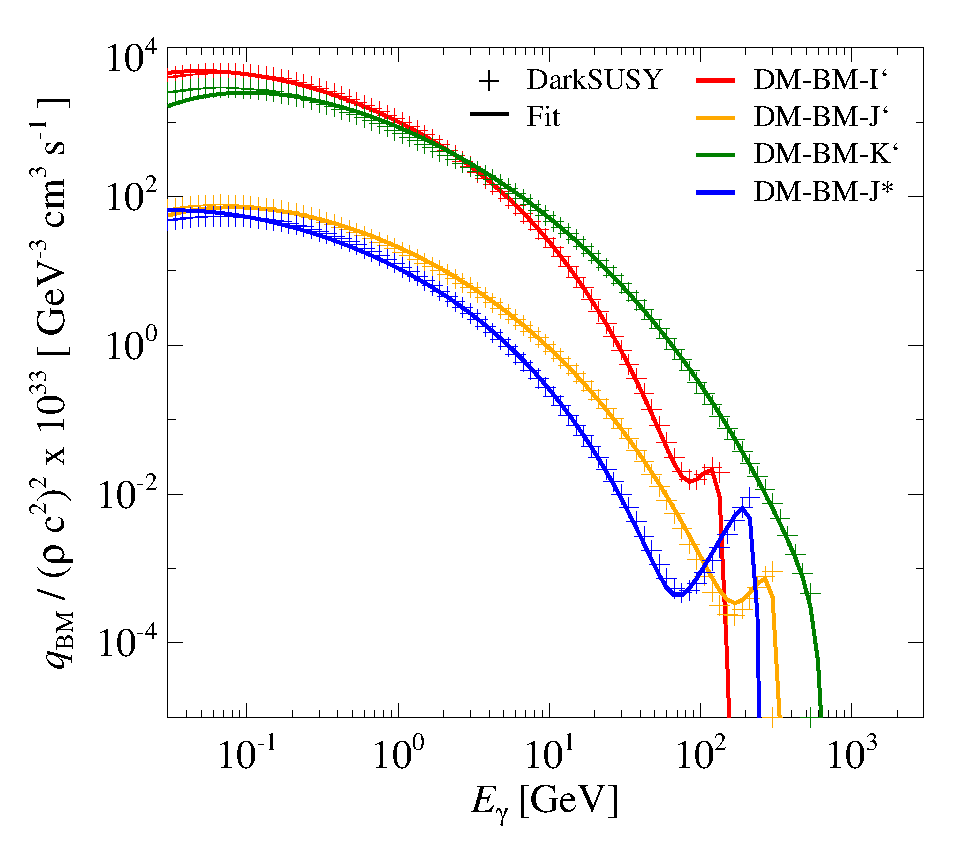
\includegraphics[width=0.49\columnwidth]{figures/fit.ds.flux.eps}
 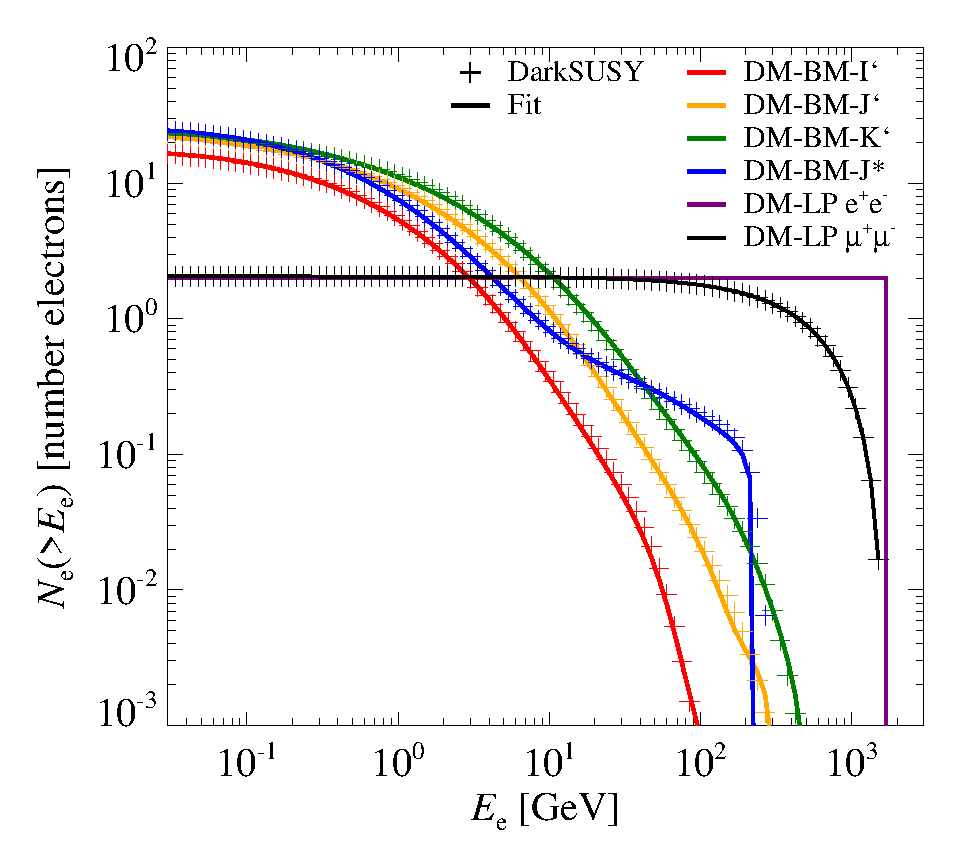
\includegraphics[width=0.49\columnwidth]{figures/fit.epflux.int.eps}
\caption{\it The underlying source functions for different DM
  models. Crosses show the simulated data from DarkSUSY and the solid
  lines show the fit to the data using Eq.... LEFT PANEL: normalized
  differential continuum spectra for four different DM benchmark (BM)
  models; $\Ip$ model (red), $\Jp$ (orange), $\Kp$ (green), and
  $\Js$ (blue). RIGHT PANEL: number of electron and positron per DM
  annihilation above the electron energy $\ee$ for different dark
  matter models; $\Ip$ BM model (red), $\Jp$ BM model (orange),
  $\Kp$ BM model (green), and $\Js$ BM model (blue), leptophilic (LP)
  DM annihilating into electrons and positrons (purple), and LP DM
  annihilating into muons (black).}
 \label{fig:q_DM}
\end{minipage}
\end{figure*}
Only LP models have energetic enough CRe such that IC emission
powerful to either constrain or be detected

similar shape for BM continuum models


\begin{figure}%[t]
 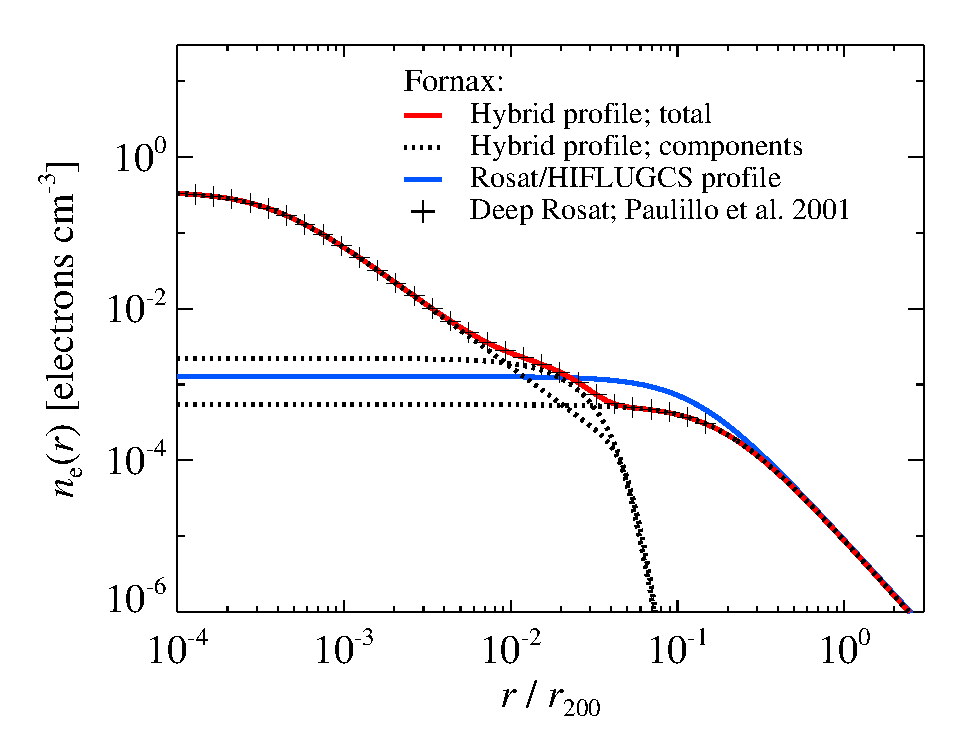
\includegraphics[width=0.99\columnwidth]{figures/dens.fornax.eps}
\caption{\it Comparing different electron number density profiles for
  the Fornax cluster. Black crosses show the density profile inferred
  from deprojected Chandra and Rosat X-ray surface brightness
  observations CITE. The total hybrid profile shown by the red solid
  line represent the best fit to the data, where the fitted individual
  density components are shown by the black dotted lines. The blue
  solid line show the single beta density profile inferred from the
  HIFLUGCS catalogue. Due to insufficient sensitivity to the outer part
  in the plotted data, we infer the outer slope found in the HIFLUGCS
  catalogue.}
 \label{fig:dens_fornax}
\end{figure}




\begin{figure*}%[t]
\begin{minipage}{2.0\columnwidth}
 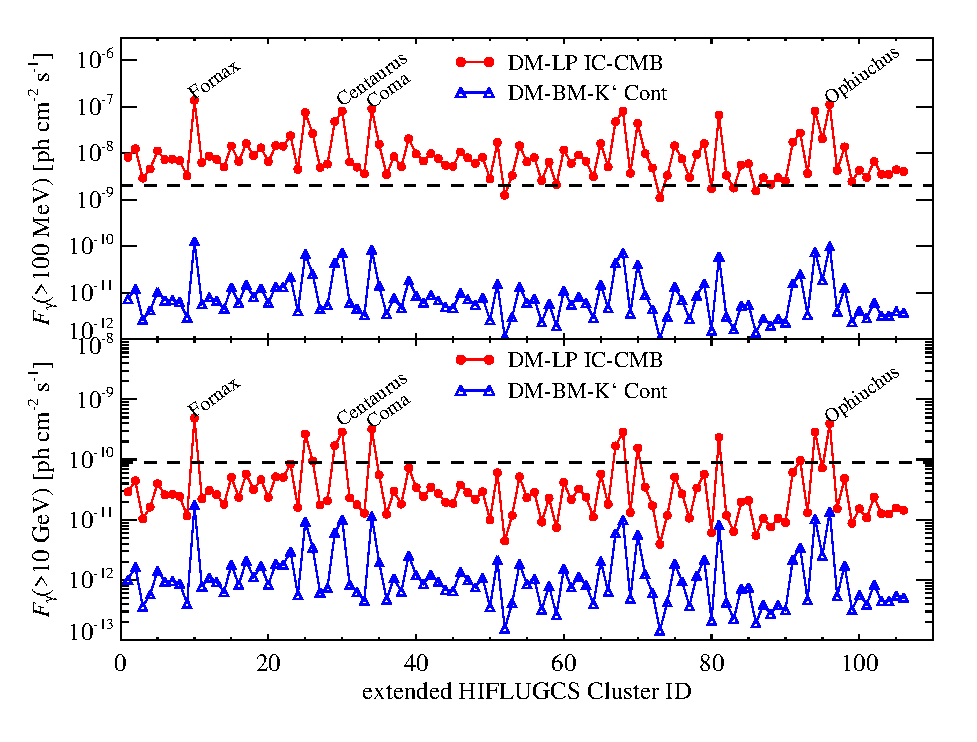
\includegraphics[width=0.99\columnwidth]{figures/Flux.comp.DM.eps}
\caption{\it Comparing the flux from clusters in the extended HIFLUGCS
  catalogue. We show the energy integrated gamma-ray fluxes derived
  from both leptophilic DM that result in inverse Compton upscattered
  CMB photons (red), and the continuum emission from the DM $\Kp$
  benchmark model (blue). The fluxes are calculated within $\rvir$
  for each of the 106 clusters included in the extended HIFLUGCS
  catalogue, and are derived using a single beta profile for each
  cluster's gas density profile (see text for details). The upper
  panel show the energy integrated flux above 100~MeV and the lower
  panel above 10~GeV, both as a function of HIFLUGCS cluster ID. The
  name of the four brightest clusters are written out, where Fornax
  and M49 are the brightest targets.}
 \label{fig21}
\end{minipage}
\end{figure*}


\end{document}
